\documentclass[11pt,a4paper]{article}
\usepackage[utf8]{inputenc}
\usepackage{amsmath}
\usepackage{amsfonts}
\usepackage{amssymb}
\usepackage{graphicx}
\usepackage[margin=1.00in]{geometry}
\usepackage{csquotes}
\usepackage{fancyhdr}
\usepackage{caption}
\usepackage{rotating}
\usepackage[nottoc]{tocbibind}
\usepackage[flushleft]{threeparttable}
\usepackage{lscape}
\usepackage{longtable}
\usepackage{booktabs}
\usepackage{wrapfig}
\usepackage[onehalfspacing]{setspace}
\usepackage[colorlinks=true, allcolors=blue]{hyperref}
\usepackage[
backend=bibtex,  % don't use "biber"!
style=authoryear-icomp, 
isbn=false,url=false,eprint=false,
sorting=nyt,sortcites=false,date=year
  ]{biblatex} 

%\setlength{\parskip}{0.25em}  % set space between paragraphs
\newcommand\fnote[1]{\captionsetup{font=footnotesize}\caption*{#1}}  % add notes to figures

\AtEveryBibitem{%
  \clearfield{note}%
}

\addbibresource{refs.bib} 

\begin{document}
\begin{titlepage}
	\centering
	\vspace*{1.5cm}
	\hrulefill\\
	\vspace{0.5cm}
	{\scshape\LARGE The Relationship Between Sibling Size and Educational Attainment of Children: Evidence from South Africa\par}
	\vspace{0.5cm}
	\hrulefill\\
	\vspace{1.5cm}

	{\normalsize\itshape A thesis submitted in partial fulfilment of the requirements for the degree of\par}
	
	\vspace{0.6cm}
	
	{\normalsize\itshape Master of Science \\ \vspace{0.2cm} in \\ \vspace{0.2cm} Economics for Development\par}
	
	\vspace{1.2cm}
	{\normalsize By \par}
	
	\vspace{1.2cm}
	{\large\itshape Name}
	
	\vspace{4pt}
	{\normalsize SID}
	
	\vspace{0.8cm}
	{\large\itshape Supervisor: Supervisor Name \par}
	
	\vspace{0.8cm}
	{\normalsize Department of International Development \\ \vspace{4pt}
	University of Oxford \\ \vspace{4pt}
	United Kingdom}
	
	\vspace{2.8cm}
	{\normalsize May 2022 \par}

\end{titlepage}

\pagenumbering{roman}

%\section*{Disclaimers}
%\input{disclaimer}
%\pagebreak
%\addcontentsline{toc}{chapter}{Abstract}
\begin{abstract}
\phantomsection % required if using hyperref
\addcontentsline{toc}{section}{\abstractname}
   Children who are raised in large families are observed to end up with less education than those from smaller families. A longstanding question in research on fertility is whether this observed negative correlation between sibling size and educational outcomes for children is causal. Using census data from South Africa, this study investigates the effect of family size on the educational attainment of children. Results from OLS regression point to the expected negative association. On the other hand, 2SLS estimates, using the birth of twins and sibling sex composition as instruments for the number of children, show no effect of fertility. Heterogeneity analysis suggests that this null effect holds in virtually all subpopulations with different sociodemographic characteristics. The results are consistent in showing that sibship size has no adverse effects on the educational attainment of children in South Africa.
\end{abstract}
\pagebreak

%\begin{center}
%\section*{Acknowledgements}
%\end{center}
%Thank everyone.
%\pagebreak

\tableofcontents
\pagebreak

\listoffigures
\listoftables
\pagebreak

\pagenumbering{arabic}


\section{Introduction}

The question of how family size affects outcomes for children has received considerable attention in the literature on fertility. The quantity-quality model, introduced by \textcite{Becker1960} and formalized in \textcite{Becker1973} and \textcite{Becker1976}, predicts that there is a trade-off between the number (quantity) of children and their “quality”. Using a utility maximization framework, the model shows that the cost or shadow price of quality increases as the number of children increases, and vice versa; this generates a trade-off between quality and quantity. One implication of this is that an increase in the number of children, keeping other factors fixed, will lower investment per child and result in children of lower quality.

Early empirical evidence on the quantity-quality relationship relied on showing a negative association between family size and outcomes for children (usually education).  However, taking these results to be evidence of a causal relationship is challenging because family size is endogenous; the number of children that parents desire to have is related to both observed and unobserved characteristics of the parents that also affect child outcomes \parencite{Black2010}. For instance, childbearing decisions are affected by the education of the parents, their earning potential, career ambition, lifestyle, and expectations about the benefits and costs of having a child \parencite{Angrist2006,oberg_casual_2021}. These are factors that also affect how much parents invest in the human capital of their children. Since most of these factors are unobserved or even unobservable, naïve attempts to estimate effect, such as ordinary least squares (OLS) regression, are likely to suffer from omitted variable bias \parencite{oberg_casual_2021}.

Studies that tried to uncover the causal effect of fertility on individual outcomes have therefore tried to exploit “natural experiments” that lead to an exogeneous increase in family size. The two well known examples of such natural experiments used as the basis for instrumental variables estimation in the literature are the birth of twins and the sex composition of older siblings (given a preference for mixed-sex siblings, parents are more likely to have another child if the sex of the first two/three children is the same). However, the majority of previous research that use either or both of these instruments were conducted in a high-income or middle-income country setting. Despite the fact that family planning policies are a more important issue in poorer countries, there is a paucity of relevant empirical evidence coming from these countries. In particular, there are very few studies on this topic from Africa, largely due to the lack of data. 

This study attempts to fill this gap by providing empirical evidence on the effect of sibling size on the educational attainment of children using census data from South Africa. Following the literature, I used both the occurrence of twin births and the sex composition of children in earlier births to instrument for family size. For the twins instrument, I considered parity specific twin births (twins at second birth and twins at third birth), and looked at outcomes for non-twin older children. This gave rise to two samples of school aged children: firstborns in families with at least two kids (called the 2+ sample) and first and second-born siblings in families with at least three children (called the 3+ sample). Similarly, the sex composition instrument was taken to be an indicator for the matching of the sexes of the first two children (for the 2+ sample) and the first three children (for the 3+ sample). First stage results show that both the occurrence of twin births and the sameness of sex in earlier births significantly increase the number of children. This holds for both the 2+ and the 3+ samples and in all the subsamples I considered.

The use of multiple instruments for the number of children is not common in the literature. Given the fact that the results from the two types of instruments have distinct features, this approach offers an advantage over studies that use a single instrument. Two important differences about the effects captured by the two instruments are worth pointing out. First, each instrument captures an effect for different segments of the population. This follows from the fact that any estimate that employs IV strategy captures the effect on individuals affected by that instrument \parencite{imbens_identification_1994}. These individuals are called the \enquote{compliers} \parencite{angrist_identification_1996}. It turns out that the group of compliers for twins and sex composition instruments are different. As will be argued later, twins instruments identify the effect of treatment on the whole population of the nontreated, whereas the compliant population for the same sex instrument is less than complete \parencite{Angrist2006,Angrist2009}. Second, as will be explained below, each instrument captures a causal effect over different ranges of sibling size. In particular, the twins instrument measures the effect of fertility at parities closer to the parity of the occurrence of twins. The same sex instrument, on the other hand, captures an effect over wider parities. 

Moreover, the two instruments are potentially subject to different types of omitted variable biases. For example, the likelihood of occurrence of twins vary with the characteristics of the mother such as age at birth, ethnicity, and health seeking behaviour. But such concerns do not arise with the same sex instrument. Instead, a challenge to the exclusion restriction with respect to the same sex IV is the possibility of gender-specific economies of scale that could reinforce child quality investments when parents have children of the same sex (Rosenzweig and Wolpin, 2000). This fact highlights a further potential advantage of using multiple instruments for family size: given the different types of endogeneity threats that the two instruments face, a comparison of the estimates using each IV can serve as a specification check \parencite{angrist_multiple_2010}.

Because of limitations on the data, the study focuses on immediate short run outcomes that relate to the schooling of children. In particular, it focuses on the grade achievement of children by the time of the census. Two variables that measure educational attainment were constructed taking into account institutional factors that could cause a variation in the grade level achieved by a child at a particular age. The first is an educational attainment index, a continuous variable that measures whether each child is at, above, or below the “appropriate” grade, and the second is an indicator for whether the child is lagging behind in grade relative to his/her peers. Moreover, two more intermediate variables were considered: whether the child attends a private school and the labour force participation status of the mother. These can be considered as inputs into child quality that reflect investment in children’s human capital \parencite{caceres-delpiano_impacts_2006}.

Results from OLS regression point to a negative correlation between family size and children’s educational attainment. However, 2SLS regression estimates using both twins and sex composition instruments show that sibling size has no effect on the educational attainment of children and other intermediate outcomes. Heterogeneity analysis conducted using generalized random forests \parencite{Athey2019} indicates this result holds across different subsamples with different sociodemographic characteristics. These findings are consistent with results from previous studies that find a negative association but no negative effect when using one or both of these instruments \parencite[see, for example,][]{Black2005,Black2010,caceres-delpiano_impacts_2006,angrist_multiple_2010,bhalotra_twin_2020}.\footnote{See also the reviews in \textcite{clarke_children_2018} and \textcite{oberg_casual_2021}.} Hence, this paper is the latest in a growing body of empirical literature that challenge the existence of a quantity-quality trade-off.

The paper proceeds as follows. Section II describes the data and samples used, the outcome variables, and the empirical framework for the IV strategy. Then, Section III discusses the results, addresses challenges to validity, and presents findings from heterogeneity analysis that were conducted using generalized random forests. Finally, Section IV concludes.


\section{Data and Methods}

The data comes from the 10\% public use sample of the 2011 South African Census. The micro data at the individual level has observations for each person within a household from all nine provinces of South Africa. I retained only sons or daughters in each household whose biological parents were alive by the time of the census and matched them with data on their mothers. After identifying the order of birth among two or more siblings using their dates of birth, I selected those observations where the age of the firstborn child is less than or equal to 18. Finally, two groups of samples were used in the final analysis. The next subsection discusses these in detail.

\subsection{The 2+ and 3+ samples}

The 2+ sample consists of only firstborn children with one or more siblings (so the total number of children per mother would be two or more). I selected only firstborns aged 8 to 18.\footnote{ South Africa has a compulsory schooling law where children who have turned 6 by June 30 are required to attend grade 1 (see \url{https://www.education.gov.za/Informationfor/ParentsandGuardians/SchoolAdmissions.aspx}). To look at 8 year olds and above would allow me to observe variations in educational achievement and grade retention. }  The twins IV (Twins2) in this sample is an indicator for whether the second birth was a multiple birth or not. But I have excluded firstborns who are twins themselves because of the special characteristics of twins that could confound results. Hence, all firstborns in this sample are singletons. Similarly, the same sex IV (SameSex12) is an indicator for whether the sex of the first and second births are the same. In order to look at the effect by gender, I disaggregated this into two separate indicators: whether the first two births were both boys (Boy12) or both girls (Girl12).\footnote{ The sum of Boy12 and Girl12 gives the SameSex12 dummy, i.e., SameSex12 = Boy12 + Girl12. }  

The first two columns of \autoref{tab:01} present summary statistics on the variables in the 2+ sample. The sample consists of almost 95,000 firstborns and has a balanced sex composition. The average number of kids is 2.7 and the mean age of the firstborns is 13. About three-quarters of the observations belong to Black African mothers, while coloured and white mothers each account for approximately 11\%. The rate of occurrence of twins in the second birth is 1\%. On the other hand, about 52\% had a sibling of the same gender from second birth. Given that 50\% of the sample are males, we have an almost equal proportion of matching first two births for each gender: 26.1\% for boys and 25.5\% for girls. 

The 3+ sample is a subsample of the 2+ sample, where both non-twin first and second-born kids with one or more siblings are included. Here also, I selected children aged 8 to 18 since I can only observe variations in schooling outcomes for kids aged 8 or older. The twins IV in this sample (Twins3) is a dummy for whether the third birth was a twin birth or not. The same sex IV, on the other hand, is an indicator for whether the first three kids were of the same sex. This is termed SameSex123. As in the 2+ sample, I have disaggregated this indicator into two separate indicators based on the sex of children in the first three births. The Boy123 and Girl123 are indicators for whether the first three children are all boys or all girls, respectively. 

Columns 3-6 of \autoref{tab:01} presents summary statistics on the 3+ sample. Columns 3 and 4 focus only on firstborns while columns 5 and 6 include both first and second-borns. There is no substantial difference across many of the variables between the firstborns in the 3+ sample and their counterparts in the 2+ sample. A similar result follows when looking at the entire 3+ sample (i.e., both first and second-borns; $ N = 57,358 $). The average family size in this sample is 3.6 and the average age of the children is 13. Just as in the 2+ sample, we have an almost perfectly balanced sex composition. The twin rate at the third birth, 1.3\%, is a little higher than in the 2+ sample. About 27\% of the observations are in households where the first three births are of the same sex. Again, this is well balanced across the two sexes (about 13.5\% each). Black African mothers now account for a larger proportion (82\%), while the share of white mothers declined to 6.1\%. One can also see that the share of mothers with no schooling is higher in the 3+ sample compared to the 2+ sample (8\% vs. 5\%).   
    

\subsection{Model Specification and Outcome Variables}
\label{section:outcomes}

The structural equation that captures the causal relationship of interest is

\begin{equation}\label{eq:01}
	y_{i} = X_{i}\boldsymbol{\beta} + \gamma n_{i} + \epsilon_{i}
\end{equation}

where $ y_{i} $ is an outcome variable, $ X_{i} $ is a vector of covariates including characteristics of the children and their mothers, and $ n_{i} $ is the total number of children (including the subject) in the household. As discussed in the introduction, because the number of children, $ n_{i} $, is endogenous, OLS estimation of \eqref{eq:01} gives a biased and inconsistent estimate of $ \gamma $. I use both the birth of twins and the sameness of sex in earlier births to instrument for family size. The rest of the current subsection discusses the outcome variables explored in the study. The next subsection has a detailed discussion on the proposed instruments.  

The study will look at the effect of sibship size on four outcome variables: (i) educational attainment, (ii) whether a kid is lagging behind in grade, (iii) whether the kid attends a private school, and (iv) the labour force participation of the mother. The first two are final outcome variables whereas the second two are considered as intermediate outcome variables \parencite{caceres-delpiano_impacts_2006}. 

Following \textcite{rosenzweig_testing_1980}, an educational attainment index was constructed by taking the ratio of the highest grade achieved by a child at the time of the census to the mean grade of all kids of the same age, month of birth, and province. The reason month of birth was chosen as a grouping variable is that laws on admission are based on the age of a child at a specific point in time during the admission year.  Hence, the month of birth is one determining factor for the variation in grade achievement of children of the same age. However, individual provinces have their own rules on registration timelines as well as implementation. From \autoref{tab:01}, the educational attainment index has a mean of 1 and a standard deviation of about 0.16 in both the 2+ and 3+ samples. \autoref{fig:01} shows a histogram of this index in both samples, which provides a more informative picture of its distribution. 

Similarly, a dummy for being left behind is constructed by comparing the highest grade of a child to the mode of the highest grade of all kids of the same age, month of birth, and province in the relevant sample. It takes a value of 1 if a child's highest grade is below the mode and 0 if it is equal to or above the mode. This essentially measures the same thing as the educational attainment index but has some advantages over the latter. Particularly, as it uses mode instead of mean, it is not affected by extreme values. But as a discrete measure it does not take into account the extent of the lagging (or progressing). It can be considered as a useful complement to the educational attainment index. According to \autoref{tab:01}, 38.6\% in the 2+ sample and 37.6\% in the 3+ sample are lagging behind using this measure. 

The third outcome variable, \enquote{private school} is a dummy for whether the child attends a private school ($ = 1 $) or a public school ($ = 0 $). Like in many countries, private schools offer better quality education and are preferred to public schools in South Africa. They are also more expensive. Thus enrollment in private school can reflect costly parental investment in the education of children. Attending a private school can also lead to better educational outcomes. The available evidence suggests that educational outcomes are better for kids attending private school, although we should be careful to interpret this as showing causation, not merely correlation \parencite{caceres-delpiano_impacts_2006}. From \autoref{tab:01}, about 9\% in the 2+ sample and 6.3\% in the 3+ sample attend private school. These might sound low but are not surprising given that private schools are expensive in South Africa.

The last outcome variable, mothers' labour force participation (Mothers' LFP) is also a dummy for whether a mother is in the labour force ($ =1 $) or not ($ =0 $). The relationship between a mother's labour market outcome and family size has been explored in many studies (\textit{cite a few studies}). As an intermediate outcome, a mother being in the labour force has ambiguous effects on child outcomes \parencite{caceres-delpiano_impacts_2006}. On the one hand, working mothers generate income that they can invest on their children, but, on the other hand spend less time caring for their children. Either way, it is an important channel between fertility and the welfare of children. According to Table 1, about 76.3\% of mothers were in the labour force in the 2+ sample, while the corresponding figure in the 3+ sample is 71.3\%.


\subsection{Instrumental Variables, Interpretation, and First Stages}
\label{section:IVs}

The main motivation behind the use of instrumental variables is to uncover a causal relationship between family size and outcomes for children. Following the potential outcomes framework, what we are trying to estimate using the birth of twins and the sex composition of siblings as natural experiments is what \textcite{Angrist1995} called the Average Causal Response (ACR). \textcite{Angrist1995} have shown that, given mild regularity assumptions, the Two Stages Least Squares (2SLS) estimates using a binary instrument $ Z $ to instrument for an endogenous variable that takes a finite set of integer values  (say $ 0, 1, \dots, J $) is the weighted average of per-unit causal effects (that is, the effect of going from 0 to 1, the effect of going from 1 to 2, and so on) along the length of an appropriately defined causal response function. More formally, let $ N_{0i} $ and $ N_{1i} $ be the potential number of children in the family if a binary instrument $ Z_{i} $ were equal to 0 and 1, respectively. The observed number of children $ n_{i} $ is then, $ n_{i} = N_{0i} + (N_{1i} - N_{0i})\cdot Z_{i} $. Similarly let $ Y_{i}(j) $ be the potential outcome as a function of $ j $, where j takes possible values for $ n_{i} $ in the set $ \{0, 1, \dots, J\} $. Only one of these potential outcomes is realized and we denote the observed outcome by $ y_{i} $. In the simplest case with no covariates, the IV estimator using a binary instrument $ Z $ gives the Wald estimator.\footnote{The interpretation of the ACR is more elaborate when covariates are added, but the basic idea is preserved. See \textcite[p.~437]{Angrist1995}.} Then,


\begin{equation}\label{eq:02}
	\beta_{w} = \dfrac{\mathbb{E}(y_{i} | Z_{i} = 1) - \mathbb{E}(y_{i} | Z_{i} = 0)}{\mathbb{E}(n_{i} | Z_{i} = 1) - \mathbb{E}(n_{i} | Z_{i} = 0)} = \sum_{j = 1}^{J} \omega_{j}\cdot \mathbb{E}(Y_{i}(j) - Y_{i}(j-1) | N_{1i} \geq j > N_{0i})
\end{equation}

where
\begin{equation}\label{eq:03}
\omega_{j} = \dfrac{\mathbb{P}(N_{1i} \geq j > N_{0i})}{\sum_{i = 1}^{J} \mathbb{P}(N_{1i} \geq i > N_{0i})}
\end{equation}
\vskip10pt

The unit causal response in \eqref{eq:02}, $ \mathbb{E}(Y_{i}(j) - Y_{i}(j-1) | N_{1i} \geq j > N_{0i}) $, is the average difference in potential outcomes for \textit{compliers} at point $ j $; that is, individuals driven by the instrument from a treatment intensity less than $ j $ to at least $ j $.\footnote{We are using the word \enquote{compliers} in the context of the treatment-effects framework outlined in \textcite{angrist_identification_1996}. See the discussion below for more explanation.} Thus, the Wald estimator, $ \beta_{w} $, is \enquote{a weighted ACR for people from families induced by an instrument to go from having fewer than $ j $ to at least $ j $ children, weighted over $ j $ by the probability of crossing this threshold} \parencite[p.~787]{angrist_multiple_2010}. The numerator in the expression for the weights $ \omega_{j} $ in \eqref{eq:03}, $ \mathbb{P}(N_{1i} \geq j > N_{0i}) $, represents the proportion of compliers at point $ j $.\footnote{Individuals with $ N_{1i} \geq j > N_{0i} $  for any $ j $ in the support of $ n_{i} $ are considered as compliers.} This is normalized by $ \sum_{i = 1}^{J} \mathbb{P}(N_{1i} \geq i > N_{0i}) $, which can be shown to be equal to the Wald first stage \parencite[see][p.~183]{Angrist2009}. That is,

\begin{equation}\label{eq:04}
\mathbb{E}(n_{i} | Z_{i} = 1) - \mathbb{E}(n_{i} | Z_{i} = 0) = \sum_{i = 1}^{J} \mathbb{P}(N_{1i} \geq i > N_{0i})
\end{equation}

There are three assumptions that lie behind the ACR theorem: (i) independence and exclusion; (ii) the existence of a first Stage; and (iii) monotonicity \parencite{Angrist2009}. The independence assumption requires that the instrument be independent of potential outcomes and potential treatment assignments. This is sometimes alternatively stated by saying that the instrument need to be as good as randomly assigned. Both the twins and same sex instruments were originally proposed as natural experiments for fertility on the ground that both are virtually randomly assigned \parencite{rosenzweig_testing_1980,angrist_children_1998}. However, this is no longer obvious because various threats to the randomness of both instruments have been pointed out in the literature (see Section~\ref{section:valid}). The exclusion assumption, on the other hand, says that the instrument used has no effect on the outcomes other than through its effect on family size.  Although this is closely related to the independence assumption, it is distinct from it. The exclusion restriction is a \enquote{a claim about a unique channel for causal effects of the instrument} \parencite[p.~153]{Angrist2009}. Again, various authors have pointed out ways in which exclusion restriction might fail to hold for both instruments. I have tried to address some of the important concerns in Section~\ref{section:valid}.\footnote{ The other important assumption needed to estimate the ACR is monotonicity. In our case, monotonicity requires that the proposed instrument moves fertility in one direction only. In particular, we assume that the potential number of children when the instrument is switched on is at least as large as it would have been when it is switched off; i.e., $ N_{1i} \geq N_{0i} $. This is automatically satisfied by the twins instrument as fertility is always increased because of a twin birth for any mother. Although rare, it is possible that monotonocity might fail to hold for the same sex instrument. For example, there could be parents who prefer children of the same sex and therefore go on to have another child if the sexes of the first two or three children are different \parencite{Huber2015}. As a partial check on monotonicity, I estimated the same sex first stage in the 2+ sample for each combination of the mother's population group, intervals of the mother's age at first birth, and the level of education of the mother. Out of the 44 first stage regressions, corresponding to the 44 cells, only three generate negative estimates and all three were insignificant. The remaining significant estimates were all positive.} 

% Consider shortening/removing this paragraph if necessary.
%The other important assumption needed to estimate the ACR is monotonicity. To understand the idea behind this assumption, we need to introduce the four mutually exclusive groups comprising of our quasi-experimental population: compliers, always takers, never takers, and defiers. These were first outlined in the treatment-effects framework of \textcite{angrist_identification_1996}.  Always takers always get treated regardless of their assignment, never takers never get treated regardless of their assignment, and compliers get treated when the instrument is switched on and don't get treated otherwise. The defiers, on the other hand, are a very strange group who get treated when the instrument is switched off and don't get treated when it is switched on. The assumption of monotonicity rules out the presence of defiers since they complicate the link between ACR and the reduced form \parencite{Angrist2009}.\footnote{\textcite{Angrist2009} discuss monotonicity in the context of the LATE framework of \textcite{imbens_identification_1994}. But this carries over directly to the ACR since the ACR is just an extension of the LATE \parencite[see][p.~181]{Angrist2009}.}  In other words, monotonicity rules out the case where the instrument pushes some people into treatment while pushing others out. In our case, monotonicity requires that the proposed instrument moves fertility in one direction only. In particular, we assume that the potential number of children when the instrument is switched on is at least as large as it would have been when it is switched off; i.e., $ N_{1i} \geq N_{0i} $. This is automatically satisfied by the twins instrument as fertility is always increased because of a twin birth for any mother. However, monotonicity need not hold for the same sex instrument as there could be parents who prefer children of the same sex and therefore go on to have another child if the sexes of the first two or three children are different \parencite{Huber2015}. In Section~\ref{section:samesx}, I discuss a partial check for monotonicity using first stage regressions. 



\subsubsection{The Twins Instrument}

%The first stage for the twins instrument is
%
%\begin{equation}\label{eq:05}
%	n_{i} = X_{i}\boldsymbol{\theta} + \delta\cdot {\rm Twins }_{i} + \xi_{i}
%\end{equation}

The twins IV used in this study is an indicator for the occurrence of twins in the second (Twins2) or third (Twins3) birth, corresponding to the 2+ and 3+ samples, respectively. There are two rationales for considering twins at a fixed parity and looking at outcomes for older non-twin children. First, it accounts for the fact that twins are more likely in a larger family. Hence, using an indicator for a twin birth at any parity as an IV will be invalid \parencite{oberg_casual_2021}. Second, looking at older children before the twin birth avoids the confounding effect from birth order that would occur after a twin birth \parencite{Black2010}. For instance, if the second birth is a twin birth, then a younger sibling will be a fourth child. So, the twin birth affects both family size and the birth order for any siblings in later births. The obvious drawback of focusing on children prior to the occurrence of twins is that it doesn't allow us to look at the effect of birth order on the children.  

Column 1 of \autoref{tab:02} reports the first stage results for the twins instruments. The results clearly show that, in both the 2+ and 3+ samples, the occurrence of twins significantly increases the number of children. A twin second birth increases the number of children by 0.83 whereas a twin third birth leads to 0.76 additional children, controlling for the other covariates in the model. These estimates remain virtually the same after controlling for same sex dummies by gender (column 4).  The twins instrument is also relevant in both samples as evident from the sufficiently large F statistics from the Wald test (963 for the 2+ sample; 484 for the 3+ sample), ruling out the case of weak instruments. 

It is important to point out what we can learn from the first stage of the twins instrument. The ACR framework introduced earlier offers two important insights on the twins identification strategy. First, the twins instrument captures the causal effect of having children on a narrow range \parencite{angrist_multiple_2010}. This is because the weights used in the calculation of $ \beta_{w} $ in \eqref{eq:02} rapidly decline with the number of births as the first stage gets weaker at higher parities. This is shown in Panel A of \autoref{fig:02}, which plots the first stage estimates, along with their 95\% confidence intervals, of the twin IVs (Twins2 and Twins3) on dummies for having at least $ j $ kids $ (j = 3, 4, \dots, 9) $.\footnote{ The coefficients and standard errors are obtained by running a simple linear regression of a dummy for having at least $ j $ kids $ (j = 3, 4, \dots, 9) $ on the twins instruments (Twins2 and Twins3). The coefficients plotted provide an estimate of $ \mathbb{P}(N_{1i} \geq j > N_{0i}) $ for $ j = 3, 4, \dots, 9 $ and their sum is equal to the (unconditional) first stage coefficient (see \eqref{eq:04}). } The first stage effects of both instruments decline sharply with more births. For example, having twins in the third birth increases the likelihood of having at least 4 kids by 0.6 while it increases the likelihood of having 5 or more kids by 0.1, with much smaller effects for 6 or more kids and no significant effects above that.  The implication of this is that the twins instrument \enquote{captures an average causal effect over a range of fertility variation that is close to the parity of the multiple birth} \parencite[p.~788]{angrist_multiple_2010}. 

The second noteworthy feature of the twins IV is that it captures the causal effect of fertility for non-treated families, i.e., families who didn't experience a multiple birth at the specified parity. In the ACR framework (or the LATE framework, in general), with the monotonicity assumption in place, the treated consist of the compliers and always takers and the non-treated consist of the compliers and never takers.\footnote{ There are four mutually exclusive groups comprising of our quasi-experimental population: compliers, always takers, never takers, and defiers. These were first outlined in the treatment-effects framework of \textcite{angrist_identification_1996}. Always takers always get treated regardless of their assignment, never takers never get treated regardless of their assignment, and compliers get treated when the instrument is switched on and don't get treated otherwise. The defiers, on the other hand, are a very strange group who get treated when the instrument is switched off and don't get treated when it is switched on. The assumption of monotonicity rules out the presence of defiers since they complicate the link between ACR and the reduced form \parencite{Angrist2009}. } An instrument \enquote{is not informative about effects on never-takers and always-takers because, by definition, treatment status for these two groups is unchanged by the instrument} \parencite[p.~158]{Angrist2009}. Hence, instruments do not usually capture the average causal effect on all of the treated or on all of the non-treated. But there are no never takers when it comes to the twins instrument since all women who have a twins second (third) birth end up with at least three (four) children. Therefore, \enquote{the parameter identified by twins instruments is the average effect on the non-treated.} \parencite[p.~788]{angrist_multiple_2010}.



\subsubsection{The Same Sex Instrument}
\label{section:samesx}

Instrumenting with the gender mix of siblings in the family was first introduced by \textcite{angrist_children_1998}, where it was used as a source of an exogenous variation in family size in investigating the labour supply response of mothers to fertility. \textcite{angrist_children_1998} explain their rationale for doing so as follows:

\begin{displayquote}[p.~451]
This instrument exploits the widely observed phenomenon of parental preferences for a mixed sibling-sex composition. In particular, parents of same-sex siblings are significantly and substantially more likely to go on to have an additional child. Because sex mix is virtually randomly assigned, a dummy for whether the sex of the second child matches the sex of the first child provides a plausible instrument for further childbearing among women with at least two children. 
\end{displayquote}

There is plenty of empirical support for the claim that parents prefer to have children of both genders and that this preference drives the decision to have additional children \parencite[e.g.,][]{norling_measuring_2018,bisbee_local_2015}. The first stage regression on the same sex dummies is also consistent with this observation. Column 2 of \autoref{tab:02} shows that, in both the 2+ and 3+ samples, the same sex dummy has a positive and statistically significant effect on the number of children.  The first stage effects of SameSex12 (in the 2+ sample) and SameSex123 (in the 3+ sample) is 0.037 and 0.051, respectively, and both are statistically significant at the 1\% level. The first stage results of the same sex dummies when disaggregated by gender reveal an interesting pattern. For the 2+ sample, the first stage effect of having two girls (0.057) is about three and a half times as large as the corresponding effect of having two boys (0.016). This gets even more pronounced in the 3+ sample: while having three boys has no statistically significant effect on the number of children, having three girls increases family size by 0.083 and the effect is statistically significant at the 1\% level of significance. It seems childbearing increases in response to having only girls more than having only boys.\footnote{ This might reveal sex preference dynamics in favour of boys, a subject which is not explored in this study. } 

The results obtained using the same sex IV should also be interpreted as an average causal response (ACR) that applies only to the subpopulation of compliers--- i.e., those families whose number of children was increased because of having had two (three) first children of the same sex. However, the ACR here differs from the one captured by the twins instrument in two important ways \parencite{angrist_multiple_2010}. First, the complier population is less than complete; not all of the non-treated are affected by the instrument. In other words, there could well be never takers, those that would not have any more children whether treated or not, among the non-treated. Second, the sex composition instrument drives fertility over a wider range of parities than the twins instrument. This is shown in Panel B of \autoref{fig:02}, which plots the first stage effects of a same-sex sibling composition on having $ j $ or more kids $ (j = 3, 4, \dots, 9) $, similar to the first stage effects discussed for the twins instruments in Panel A earlier. The effect of a same-sex sibship declines less sharply with the number of kids when compared with the corresponding effects of twin births (Panel A). This is particularly true in the 3+ sample. Panels C and D of \autoref{fig:02} plot the first stage effects of an all-male or an all-female sex composition. The plots make it is clear that the positive effect of a same-sex sibship on family size is driven by an all-girls sibship as opposed to having only boys. This suggests that an all-female sibship induces some families to keep having children at higher parities in order to achieve a more balanced sex composition. 

%This is particularly true for the Girl12 and Girl123 instruments. Panels B and C of \autoref{fig:02} show the first stage effects of an all male or an all female sex composition on having $ j $ or more kids $ (j = 3, 4, \dots, 9) $, similar to the first stage effects discussed for the twins instruments in Panel A earlier. The plots make it is clear that the positive effect of same sex sibship on family size is driven by an all-girls sibship as opposed to having only boys. More importantly, the effect of an all female sibship declines less sharply with the number of kids in both the 2+ and 3+ samples, when compared with the corresponding effects of twin births (Panel A). This suggests that an all-female sibship induces some families to keep having children at higher parities in order to achieve a more balanced sex composition. 

%Another issue that needs to be addressed is the possibility that the monotonicity assumption could be violated when using sex composition instruments. This is because, as discussed above, we cannot rule out the presence of defiers. As a partial check on monotonicity, I estimated the same sex first stage in the 2+ sample for each combination of the mother's population group, intervals of the mother's age at first birth, and the level of education of the mother. The results of the unconditional first stages along with their 95\% confidence intervals are plotted in \autoref{fig:03}. As shown in Panel A, out of the 44 first stage regressions, corresponding to the 44 cells, only three generate negative estimates and all three are insignificant.\footnote{ I omitted 4 cells with less than 50 observations in them. } Panels B and C show the corresponding results for the Boy12 and Girl12 instruments, respectively. The results for Girl12 are similar to that of SameSex12, and the first stage effect is stronger than for Boy12 in each cell. The results for Boy12 are less robust and contains more number of negative estimates. But only two of the negative estimates are marginally significant at the 5\% level, while the rest are insignificant. Overall, the results give no indication for the presence of defiers whose fertility decision is negatively impacted by same-sex siblings in earlier births.








\section{Results and Discussions}
\label{section:results}

In this section, I present and discuss the main regression results on the effect of the number of children on different outcomes. I will first present and discuss the main regression estimates found using the whole population of firstborns (2+ sample) and the population of first- and second-borns (3+ sample), which are reported in \autoref{tab:main-res}. The subsections that follow discuss possible challenges to the validity of the instruments used and whether there is effect heterogeneity with respect to the characteristics of the mother.


%Tex File: D:/R_projects/MScED_Dissertation/tex/tables/main-res.tex

% Date and time: Fri, May 13, 2022 - 2:58:39 PM
\begin{sidewaystable}[!htbp] \centering 
  \caption{OLS and 2SLS Estimates of The Effect of The Number of Children} 
  \label{tab:main-res} 
\begin{threeparttable}
\begin{tabular}{@{\extracolsep{5pt}}lcccccccc} 
\\[-1.8ex]\hline 
\hline \\[-1.8ex] 
 & \multicolumn{4}{c}{2+ Sample} & \multicolumn{4}{c}{3+ Sample} \\
\cline{2-5}  \cline{6-9} \\
 & OLS & \multicolumn{3}{c}{2SLS} & OLS & \multicolumn{3}{c}{2SLS} \\ 
\cline{3-5}  \cline{7-9} \\[-1.8ex]
\\[-1.8ex] & (1) & (2) & (3) & (4) & (5) & (6) & (7) & (8)\\ 
\hline \\[-1.8ex] 
 Educational Attainment & $-$0.006$^{***}$ & 0.005 & $-$0.013 & 0.004 & $-$0.008$^{***}$ & 0.012 & 0.052$^{*}$ & 0.016$^{*}$ \\ 
  & (0.001) & (0.006) & (0.023) & (0.006) & (0.001) & (0.009) & (0.028) & (0.008) \\ 
  & & & & & & & & \\ 
 Left Behind & 0.023$^{***}$ & $-$0.004 & 0.084 & 0.001 & 0.025$^{***}$ & $-$0.025 & $-$0.025 & $-$0.025 \\ 
  & (0.002) & (0.019) & (0.074) & (0.018) & (0.003) & (0.025) & (0.078) & (0.024) \\ 
  & & & & & & & & \\ 
 Private School & $-$0.003$^{***}$ & $-$0.017 & $-$0.021 & $-$0.017$^{*}$ & $-$0.003$^{**}$ & 0.010 & $-$0.025 & 0.007 \\ 
  & (0.001) & (0.011) & (0.041) & (0.010) & (0.001) & (0.016) & (0.047) & (0.015) \\ 
  & & & & & & & & \\ 
 Mothers LFP & $-$0.019$^{***}$ & $-$0.021 & 0.027 & $-$0.019 & $-$0.023$^{***}$ & 0.038 & 0.112 & 0.045 \\ 
  & (0.002) & (0.016) & (0.061) & (0.015) & (0.003) & (0.030) & (0.093) & (0.028) \\ 
  & & & & & & & & \\ 
\hline \\[-1.8ex] 
IV used & - & Twins2 & Boy12 & Twins2, Boy12 & - & Twins3 & Boy123 & Twins3, Boy123 \\ 
  &   &   & Girl12 & Girl12 &   &   & Girl123 & Girl123 \\ 
\hline 
\hline \\[-1.8ex] 
\end{tabular} 
\begin{tablenotes}
\footnotesize
\item \textit{Notes:} Covariates for all models include age 
(in months) and sex of child, mother's characteristics (education, ethnicity, age during
census, age at first birth, and income range), dummies for districts, and a dummy for whether the father 
resides in the household. The regressions for the 3+ sample are clustered by mother's ID.
The regressions using the SameSex12 and SameSex123 instruments were excluded for reasons 
of space. The results are qualitatively similar to the ones in columns 3 and 7, 
respectively, and are available upon request. Robust standard errors are in parentheses. 
*** Significant at 1\%, ** Significant at 5\%, * Significant at 10\%.
\end{tablenotes}
\end{threeparttable}
\end{sidewaystable} 





\autoref{tab:main-res} presents OLS and 2SLS estimates of the effect of the number of children on the four outcome variables discussed in Section \ref{section:outcomes}. OLS results, reported in column 1 (for the 2+ sample) and column 5 (for the 3+ sample), point to the expected negative association between family size and favourable outcomes.These results correspond to the standard pattern: children who grow up in larger families have lower educational attainment, are more likely to be left behind in school, and are less likely to attend private school. Mothers are also less likely to participate in the labour market when they have many children. It is also important to point out that these estimates are very precise: their standard errors range from .001 to .003. However, these results are only indicative and, in the presence of possible endogeneity of family size, cannot be taken as showing causality.

In contrast to the OLS results, 2SLS estimates consistently point to a statistically insignificant or even positive effects of family size. The 2SLS results using Twins instruments are shown in column 2 (for the 2+ sample) and column 6 (for the 3+ sample) of \autoref{tab:main-res}. All of the estimates are statistically insignificant at conventional levels and even some have unexpected signs. For example, the effect on the educational attainment index in the 2+ sample using Twins2 as an IV is .005 (se = .006) while the corresponding effect in the 3+ sample (using Twins3 as an IV) is .012 (se = .009). Similarly, the 2SLS estimates of the impact on the dummy variable \enquote{Left Behind} are statistically insignificant and have the unexpected signs in both the 2+ and 3+ samples. The lack of statistical significance using twins instruments also extend to the variables that relate to child investment, that is, private school attendance and the mother's labour force participation. 

Similar results hold when using sex composition instruments. 2SLS estimates using both Boy12 and Girl12 instruments (column 3 of \autoref{tab:main-res}) show no effect of the number of children on any of the outcomes. Similar results hold in the 3+ sample when using Boy123 and Girl123 instruments together (column 7 of \autoref{tab:main-res}). The only exception is the effect on educational attainment [0.052 (se = 0.028)], which surprisingly, has an unexpected sign and is statistically significant only at the 10\% level. The results for the probability of being left behind in the 3+ sample and mothers' labour force participation in both samples, although insignificant, also have the opposite signs to the OLS estimates. It is also worth noting that the standard errors of the estimates obtained using sex composition instruments are substantially higher than the corresponding standard errors for the twins instruments in all of the estimated models.

Columns 4 and 8 of \autoref{tab:main-res} report 2SLS results using an instrument list that combines the twins and sex composition instruments in each sample. The purpose of combining these two different sets of instruments is to increase precision and thereby produce a single more efficient IV estimate \parencite{angrist_multiple_2010}. Indeed, the standard errors of the estimates in column 4 (2+ sample) and column 8 (3+ sample) are lower than the corresponding estimates using each group of instruments separately (columns 2 and 3 for the 2+ sample; and columns 6 and 7 for the 3+ sample). The estimates obtained using the combined instruments bolsters the null results that is obtained using each instrument set separately: none of the estimates obtained are statistically significant at the 5\% level and only two results are significant at the 10\% level. The estimate for the effect on educational attainment in the 3+ sample [0.016 (se = 0.008)], although significant at the 10\% level, has an unexpected sign. The effect on private school attendance in the 2+ sample, which is $ -0.017 $ (se = 0.010), is the only other estimate that is significant at the 10\% level.

As discussed in Section \ref{section:IVs}, the two sets of instruments capture an average causal response for different subpopulation of compliers. We have also shown that each instrument shifts the fertility distribution very differently (see \autoref{fig:acrs}). Now, given the similar set of 2SLS estimates they generate, one wonders if these results are pointing to a homogenous effect, i.e., a common family size effect of zero for just about everybody. I conducted an overidentification test to formally test the equality of the 2SLS estimates generated by the two sets of instruments. The test results (not presented, but available upon request) show that we cannot reject the null of equality of the estimates for the two instrument sets across all of the outcomes in both samples. In this setting, the traditional overidentification test becomes a formal test for treatment effect homogeneity.\footnote{ Homogeneity of results is also a strong indication of the external validity of the results \parencite[see][p.~776]{angrist_multiple_2010}. Thus, the overidentification test also serves to assess, to some extent, external validity. } But, as \textcite[p.~167]{Angrist2009} point out, this requires maintaining the hypothesis that all instruments in the overidentified model are valid, a topic we turn to next.


\subsection{Validity of the Instruments}
\label{section:valid}

A very important consideration in any IV study is validity. Following the ACR framework, anything that affect the randomness of our instruments and/or causes the exclusion restriction to fail is a threat to validity. In such a case, 2SLS estimates become biased and inconsistent. In this subsection I discuss various challenges to the randomness of both instruments and ways I tried to address them.

One concern with the randomness of twin births is that it might be related to family background characteristics. There is a common finding that older mothers are more likely to give birth to twins than younger mothers. I find this to be also the case in the 2+ sample but not in the 3+ sample. Mothers who give birth to twins during their second birth are about a year older at first birth compared to mothers who don't in the 2+ sample. In order to address this, I run separate regressions (both OLS and 2SLS) after splitting the 2+ sample based on intervals of the mother's age at first birth. The estimates, along with their 95\% confidence intervals are plotted in \autoref{fig:age-mods}. The general picture reveals that the results remain qualitatively the same across all age ranges, suggesting that systematic biases due to the age of the mother is not a concern. In particular, the 2SLS estimates for the \enquote{older mothers} ($ \geq 30 $ years old at first birth) as well as the \enquote{younger mothers} (less than 30 years old at first birth) show no statistically significant impact of the number of children on virtually any of the outcomes. The only exception is the effect on educational attainment for the 30+ sample, but this is barely significant (imprecisely estimated) and has the opposite sign to the OLS estimate. 

\begin{figure}[!th]
\centering
\caption{\label{fig:age-mods}Plot of Coefficient Estimates and 95\% CI by Intervals of the Mother's Age at First Birth (2$ + $ Sample)}
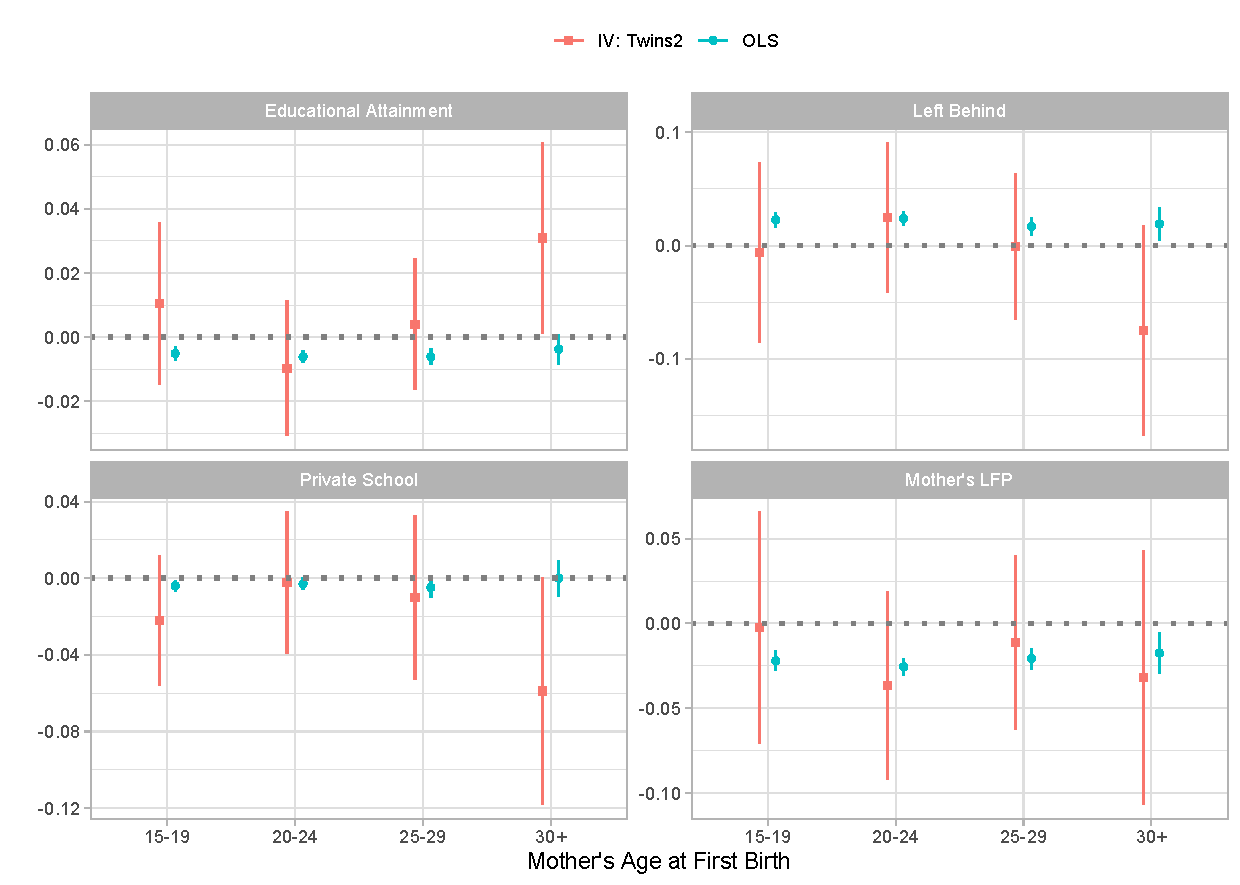
\includegraphics[width=\textwidth]{figures/age_mods.pdf}
\fnote{\textit{Notes:} Each regression was run controlling for the same set of covariates as in \autoref{tab:main-res} for the 2+ sample (see notes there). The sample sizes for each age range are as follows: 24,414 (15-19); 35,125 (20-24); 23,864 (25-29); and 10,021 (31+). Mothers who were younger than 15 at first birth were excluded from the analysis.}
\end{figure}

Another challenge to randomness of twins is the observation that mothers who use fertility enhancing treatments are more likely to have multiple births. Since the use of fertility enhancing treatments is usually unobservable, there is a potential bias from using twin births as an instrument \parencite{braakmann_reconsidering_2016}. Although availability and utilization is low, Assisted Reproductive Technologies (ARTs), such as in vitro fertilizations (IVFs), are becoming more prevalent in South Africa. In fact, South Africa has the second highest number of registered IVF centres in the whole continent in 2019 \parencite{Ombelet2019}. Studies analysing ART registry data from sub–Saharan Africa have observed high multiple pregnancy rates associated with the utilization of ART \parencite{Botha2018,Dyer2019}. There are also indications of a rise in the number of multiple births over time in our data set that could be associated with the evolution of ARTs. Using the dates of births of all respondents in the 2011 South African Census, I plotted the number of multiple births (i.e., twins, triplets, quadruplets, etc.) per 1000 live births from 1970 onwards. This is shown in \autoref{fig:line-pp}. Although there is no historical data on the utilization of ART in South Africa since its introduction in the 1980s (ART registries were established in the early 2000s), the rising trend of multiple births across all population groups is consistent with the introduction and (slow) dissemination of fertility treatments. The figure also indicates the rising disparity in twinning probabilities between white and non-white South Africans (more on this below).

%\begin{figure}[!th]
%\centering
%\caption{\label{fig:line-pp}Multiple Births Per 1000 Live Births by Mother's Population Group}
%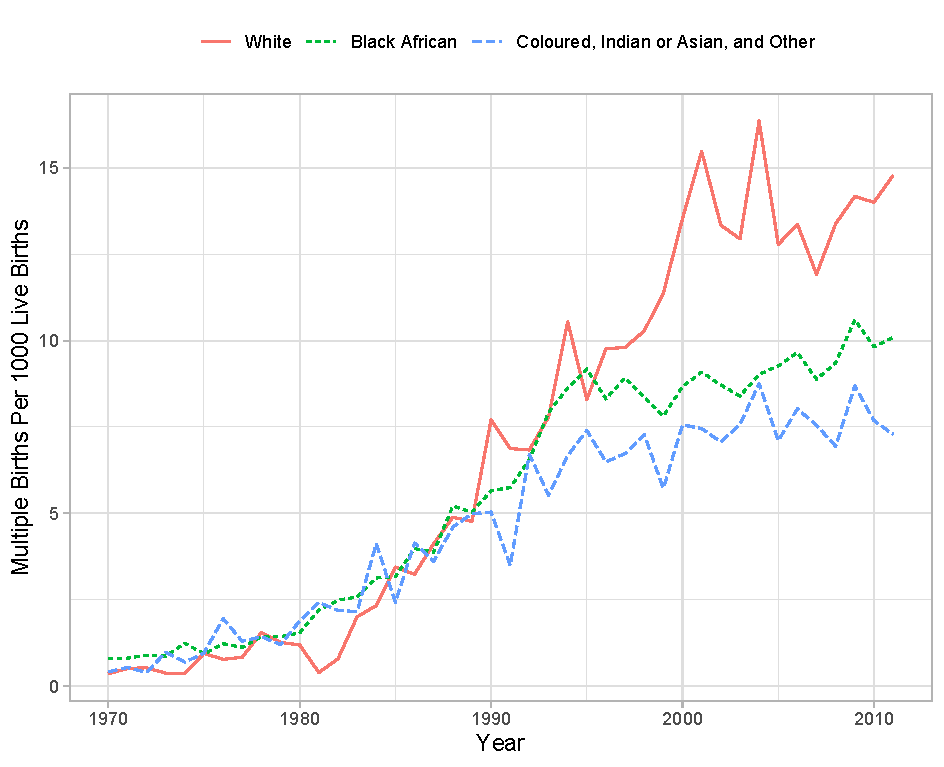
\includegraphics[width=\textwidth]{figures/line_pp.pdf}
%\end{figure}

A related threat to the randomness of twin births is the observation that the occurrence of twins is related to the mother's health and health related behaviour. \textcite{bhalotra_twin_2019} show that twinning is strongly related to morbidity, smoking status, availability of reproductive health services and other health indicators even for mothers not using fertility treatments. They also show that the education of the mother is positively associated with twinning, consistent with the hypothesis that educated women are more likely to engage in health seeking behaviour (as well as to seek fertility enhancing treatments). Although the 2011 South African census does not have data on health indicators, there are indications that twinning is more likely in subpopulations that are more likely to seek health treatments. \autoref{fig:line-pp} reveals that starting from the mid-1990s the occurrence of multiple births is systematically higher among white South Africans as compared to non-whites. This would make sense as white mothers arguably have both the awareness and the capacity with respect to utilizing health treatments, including ARTs. 

To check whether this systematic difference poses a challenge, in each sample, I estimated both OLS and 2SLS regressions using the relevant twins instrument for white and non-white families separately. The results are reported in \autoref{tab:whites-nonwhites}. As can be clearly seen, none of the 2SLS estimates are statistically significant for either whites or non-whites in both samples. Moreover, the signs of the 2SLS estimates, although insignificant and sometimes unexpected, agree for most outcomes. In general, the results are robust to division by mothers' population group, suggesting that there is no evidence of a potential bias stemming from systematic differences in the occurrence of multiple births. Perhaps, the only noteworthy difference is that the correlation between the number of children and the outcomes as captured by the OLS estimates is weaker and usually absent for whites. This, in particular, is clearly observed in the 3+ sample, where almost none of the OLS coefficients are statistically significant at conventional levels. For non-whites, on the other hand, all of the OLS coefficients have their expected signs and are highly significant. 

\textcite{rosenzweig_population_2009} point out a further challenge to the exogeneity of twin births. They argue that the occurrence of twins changes the behaviour of parents in such a way that they reallocate resources away from twins and towards older singleton children. They point out two aspects of twins that affect inter-child allocations: \enquote{(i) the closer spacing of twins, which makes investing in the average quality of the twins more costly compared with investing in non-twins, and (ii) the lower endowments of twins, which will affect the resources allocated to non-twins depending on whether parents reinforce or compensate for endowment differences across children.} \parencite[1152]{rosenzweig_population_2009}.\footnote{ Here, the lower endowment of twins refers to the fact that twins usually have lower birth weight, lower survival rate, lower cognitive achievement, and so on. } If such resource reallocation is taking place, then, they claim, estimates using twins as an instrument will be biased towards zero.

Following \textcite{angrist_multiple_2010}, I estimated reduced-form twins effects on outcomes in samples in which twins are unlikely to affect family size (i.e., there is no first stage) to see if resource reallocation is a problem. The rationale for focusing on no-first-stage samples is that because the birth of twins has no effect on family size in these subsamples, effects of confounding factors related to twinning should surface. The two subsamples with a zero first stage are those from families with closely spaced births ($ <2 $ years between the first two births) and those whose mothers were not educated, both from families with at least three children in the 2+ sample.\footnote{ These are households who are likely to have large families anyway. In such a case, the birth of twins is likely to have little or no effect on family size. }  Columns 1 and 2 in Panel A of \autoref{tab:reduced} shows that the first stage regressions in such families yield insignificant coefficient estimates at the conventional 5\% level. Panel B presents estimates of reduced form regressions for all four outcome variables using the Twin2 IV. If what \textcite{rosenzweig_population_2009} propose is true, we ought to see that older singletons have better outcomes in these no-first-stage samples. But that is simply not the case: in both subsamples, twin births have an insignificant effect (at the 5\% level) on any of the outcomes for older children. The only exception is the probability of private school attendance in the subsample of uneducated mothers (column 2). But even in this case, firstborn children have \textit{lower}, not higher, likelihood of attending private school, in defiance of the hypothesis that non-twin firstborn children are favoured. Hence, there is no evidence for a reallocation effect that could potentially confound our IV estimates.\footnote{ \textcite{Black2010} reached the same conclusion using data on the birth weight of individuals in Norway. In contrast to the critique by \textcite{rosenzweig_population_2009}, they noted that taking account of endowments actually \textit{reduces} the negative effects of family size, a result, they claimed, \enquote{is consistent with compensating rather than reinforcing parental investments} \parencite[p.~35]{Black2010}. } 
  
A similar concern with sex composition instruments is that it might be correlated with background characteristics of the parents. To test this, I estimated a regression of the same-sex instruments in each of the 2+ and 3+ samples (where the first two children are of the same-sex) on the full set of covariates, including characteristics of the mother. The results show no relationship between any of the mother’s background characteristics or other variables and the SameSex12 instrument in the 2+ sample. Only two variables (out of a total of 79) that correspond to the income group of the mother are found to be significant in the 3+ sample regression. But this is not a concern as we condition on these variables in the 2SLS estimation.

One objection to the exclusion restriction with respect to the same-sex IV is that there is a possibility of gender-specific economies of scale (for example, sharing of rooms and/or clothes) that could reinforce child quality investments when parents have children of the same-sex \parencite{clarke_children_2018}. \textcite{rosenzweig_natural_2000} point out that cost efficiencies associated with gender mix will confound the effect of an exogenous increase in the number of children with direct child-rearing cost effects on outcomes. To test this, I run reduced form regressions on subsamples with zero first stages, similar to the no-first-stage analysis for the twins instrument discussed earlier. I consider outcomes for firstborn boys in the 2+ sample, so the appropriate instrument to consider would be the Boy12 dummy. The two subsamples include mothers with less than 2 years of spacing between the first two births and those with no schooling. The results, which are reported in columns 3 and 4 of \autoref{tab:reduced}, show that there is no reduced form relation between the Boy12 instrument and any of the outcomes for the firstborn child. That is, a firstborn male child who has a younger sibling of the same gender does not appear to benefit in anyway as suggested by the same-sex cost advantage hypothesis.\footnote{ The only statistically significant effect is observed on the mother's labour force participation in the subsample with close spacing (column 3). But we are focusing here on the direct effects on the child’s outcomes. Even though there would be indirect effects, we should have seen it in the regressions where child outcomes are the dependent variables. } Hence, there is no ground to suspect a violation of the exclusion restriction based on household efficiencies related to same-sex sibships. 


\subsection{Heterogeneity Analysis}

A natural question in any causal analysis is whether the treatment effect varies with covariates, such as age, ethnicity, etc. This kind of heterogeneity analysis helps to assess the external validity of the study and allows for testing of theories on the mechanisms behind the relationships \parencite[e.g.,][]{angrist_children_1998}. Most studies that attempt to assess heterogeneity using instrumental variables regression, however, rely on a coarse subgroup analysis of the type we did in \autoref{tab:whites-nonwhites} (Whites vs. Non-Whites) or \autoref{fig:age-mods} (splitting by the mother's age at first birth). Although informative to some extent, such basic subgroup analysis is not able to identify heterogenous effects across multiple dimensions at once. Moreover, the procedure is partially ad-hoc and could sometimes lead to overfitting, as there is usually a large number of potential ways to form subgroups \parencite{Chernozhukov2018}.

To overcome this limitation and to gain deeper insights into the nature of heterogeneity in the effect of the number of children, this study implements generalized random forests (GRF). GRF, introduced by \textcite{Athey2019}, is a machine learning algorithm that extends the application of random forests to a general class of estimation methods that solve conditional moment conditions \parencite{Biewen2020}. One application of GRF is the estimation of heterogeneous treatment effects using instrumental variables.\footnote{ The method basically involves nonparametric instrumental variables regression based on random forests to estimate a (conditional) local average treatment effect. \textcite{Athey2019} provide a software implementation in R through a package called \texttt{grf}, which can easily be used to train different classes of generalized random forests, including instrumental forests. } \footnote{ Interestingly, to illustrate the application of GRF in analysing heterogeneity, \textcite{Athey2019} used data from \textcite{angrist_children_1998}'s study of the effect of family size on parental labour supply using sibling-sex composition instruments, a question closely related to the current study. } I fitted a GRF for models of three outcome variables: educational attainment of the child, the dummy for being left behind, and the dummy for private school attendance, using both the Twins2 and SameSex12 instruments in the 2+ sample. The covariates used in fitting the instrumental forests include the child's sex and age (in months), the mother's age at first birth, her age at the time of the census, education, ethnicity (Black African, White, or Coloured), martial status, employment status, and income group of the mother, and an indicator for whether the father resides in the household. I then predicted conditional local average treatment effects ($ \tau(x) $), along with their 95\% confidence interval, by varying (i) the mother’s age at first birth and her ethnicity, and (ii) the mother's education and ethnicity. The results are shown in \autoref{fig:heter1} and \autoref{fig:heter2}. The covariates not shown on the plots were set at their median values. 

Panel A of \autoref{fig:heter1} plots the effects of sibling size, instrumented using twins birth, along the dimensions of the mother's ethnicity and age at first birth. The estimated effects on all three outcomes are insignificant and do not vary along the two dimensions. The effects on educational attainment are the most precisely estimated and seem to indicate an exact null effect. \autoref{fig:heter1}B displays the corresponding estimates along the dimensions of the mother's ethnicity and level of education. Again, none of the estimates are significant for all three outcomes in any subgroup. Here also, the effects on educational attainment are the most precisely estimated but the estimates cannot be distinguished from zero for any subgroup. 

%\begin{figure}[p!]
%\centering
%\caption{\label{fig:heter1}Results of Generalized Random Forest Using Twins IV}
%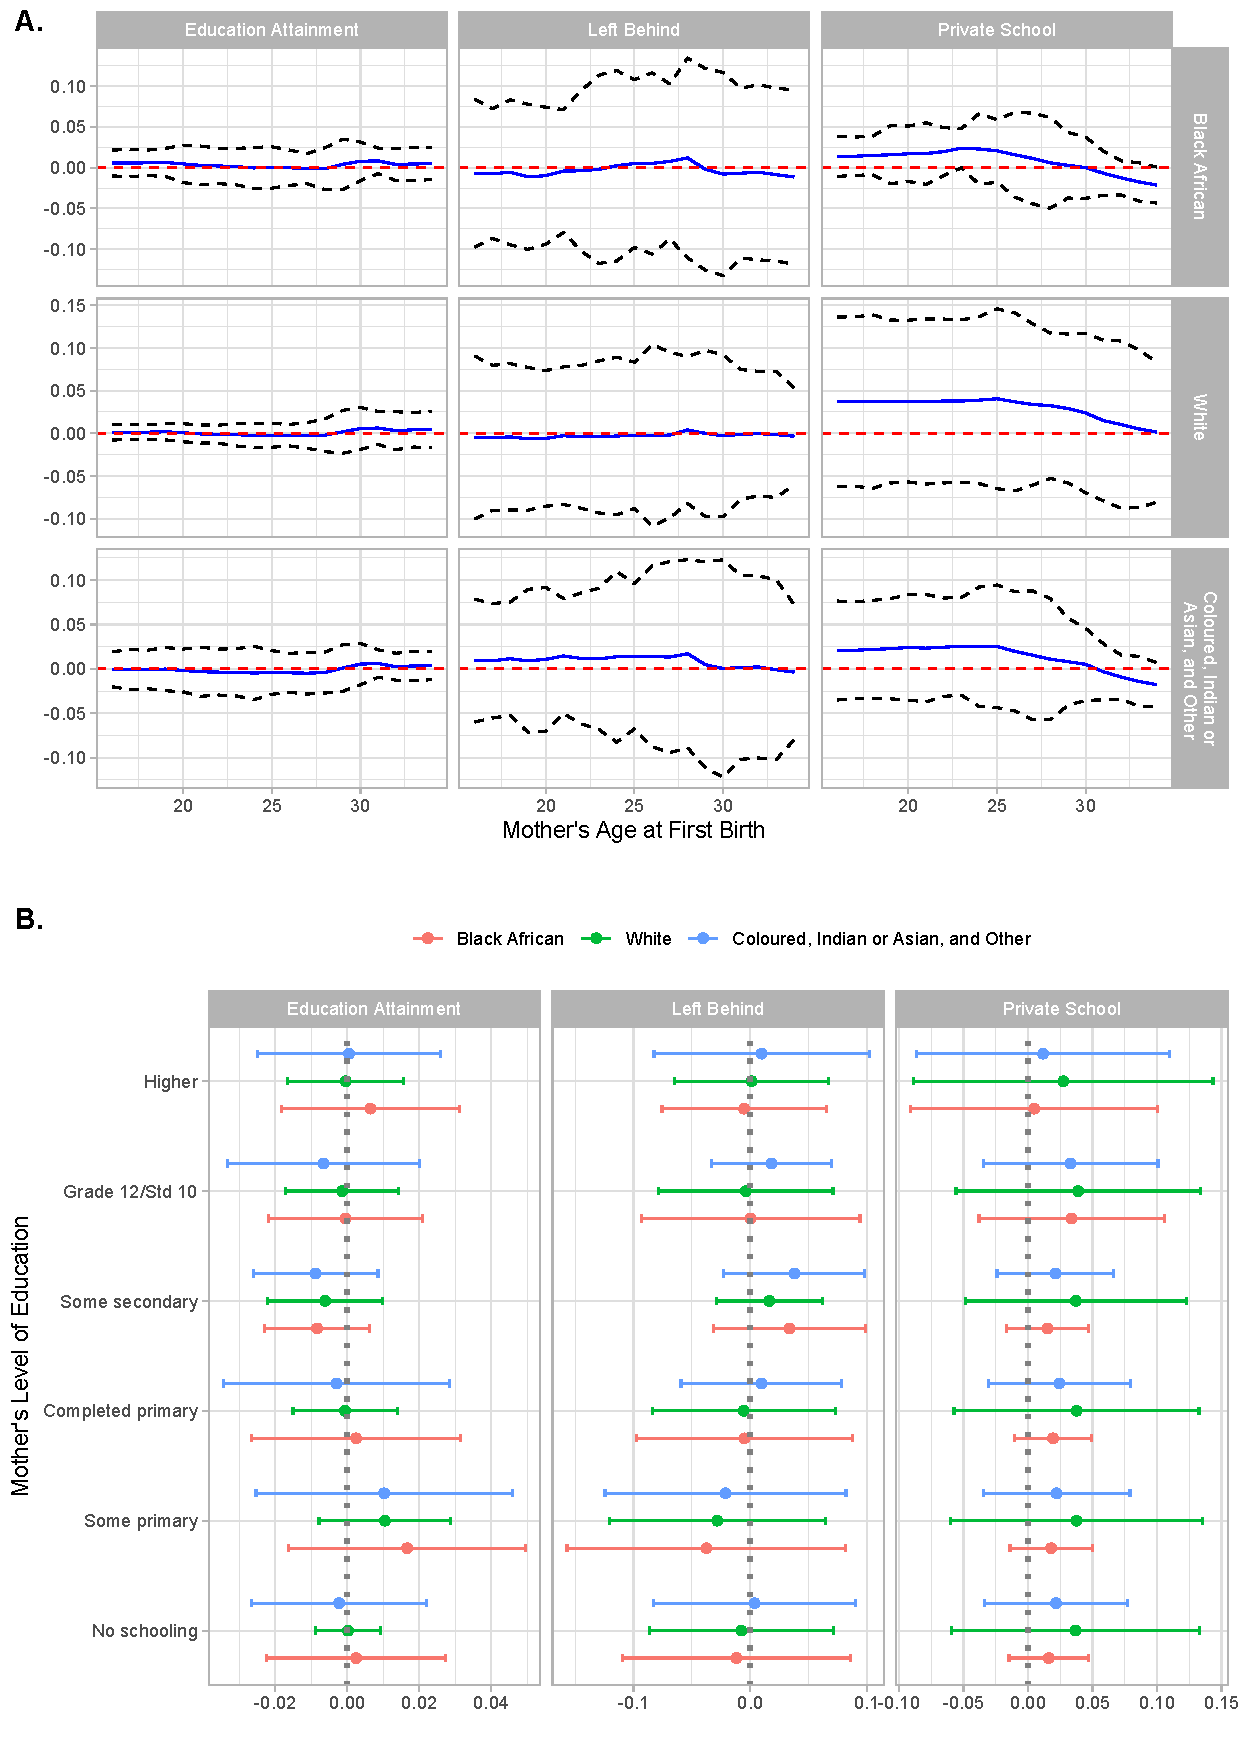
\includegraphics[width=\textwidth]{figures/heter1.pdf}
%\fnote{\textit{Notes:} The above results are based on three forests, one forest for each outcome. Tuning results suggest the default values of the parameters as optimal for each forest. Each forest is based on 5000 trees. }
%\end{figure}
%
%\begin{figure}[p!]
%\centering
%\caption{\label{fig:heter2}Results of Generalized Random Forest Using Same-Sex IV}
%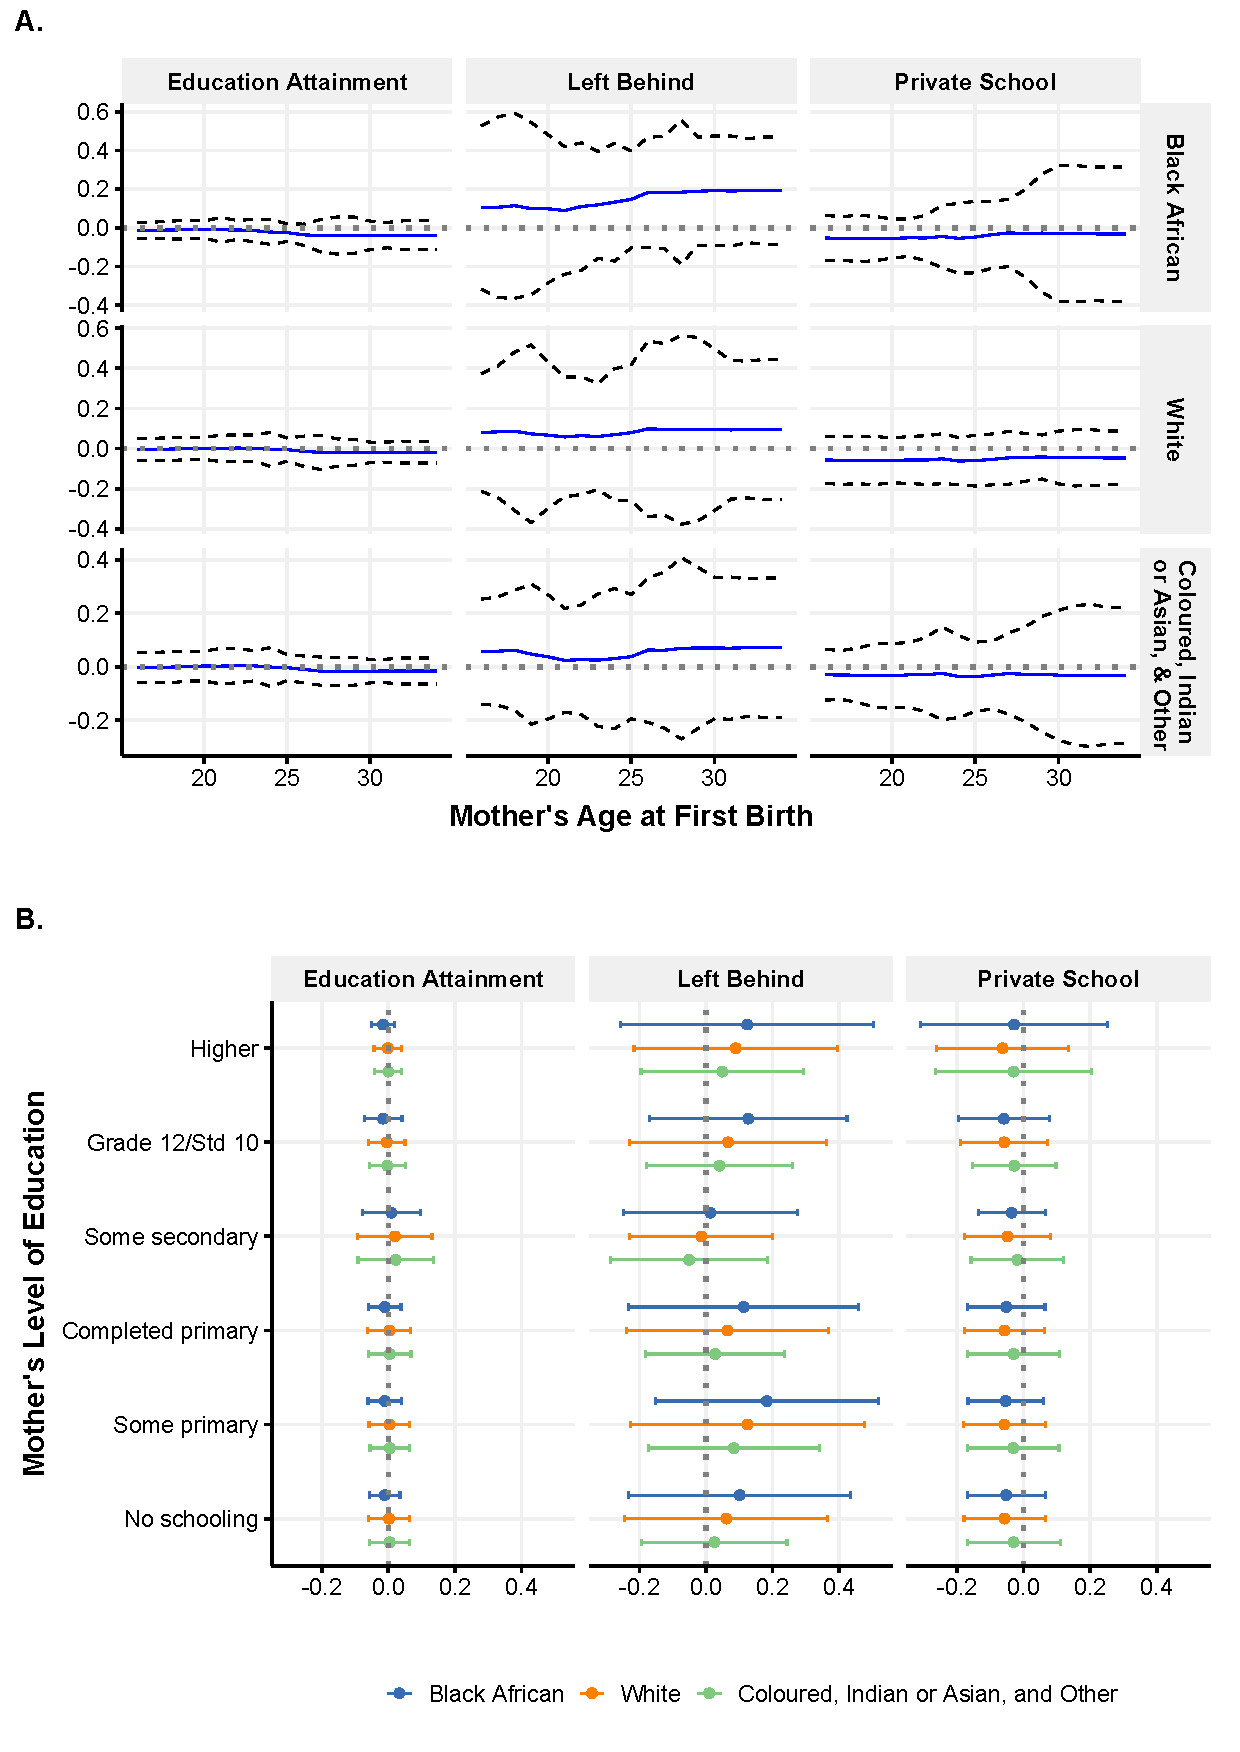
\includegraphics[width=\textwidth]{figures/heter2.pdf}
%\fnote{\textit{Notes:} The above results are based on three forests, one forest for each outcome. The parameters supplied in training each forest were chosen by tuning based on cross-validation. Each forest is based on 5000 trees. }
%\end{figure}

\autoref{fig:heter2} presents the corresponding results obtained using the same-sex instrument (SameSex12). The general pattern of the results is very similar to those presented in \autoref{fig:heter1}. \autoref{fig:heter2}A shows that the effects on educational attainment are almost null for every combination of the mother's age at first birth and her population group, though the confidence intervals are a bit wider than those shown in \autoref{fig:heter1}A. \autoref{fig:heter2}B presents results that parallel those in \autoref{fig:heter1}B. Except for minor distinctions, the results in the two plots are qualitatively identical. Again, the estimates for educational attainment are very precise and seem to indicate an exact null effect. 

In general, the results from a heterogeneity analysis presented above are remarkably consistent in showing no effect of sibling size on any of the outcomes in all the subgroups considered. The estimated effects obtained using two very different instruments (twins birth and sibling sex composition) surprisingly coincide well and in both cases not a single subgroup with a significant effect is identified. This observation bolsters the external validity of these findings; they give us more confidence that the results can be extrapolated to a different population with different characteristics. 

\section{Conclusion}
\label{section:conclude}

This study investigated whether there is a causal relationship between sibship size and the educational attainment of children using census data from South Africa. It employed an IV strategy that relied on a plausible exogenous variation in the number of children due to the birth of twins and preferences for a mixed-sibling sex composition. While both instruments exhibit a strong first-stage and OLS estimates are negative and significant, results from 2SLS regressions provide no evidence of a negative consequences of increased sibship size on educational attainment and other intermediate outcomes. Analysis of effect heterogeneity along multiple dimensions fails to find a significant impact in any of the subsamples and shows that the results do not vary with observable characteristics of the mother. These results are in line with previous research which find no or little effect of family size on child outcomes using similar approaches \parencite[e.g.,][]{Black2005,Black2010,caceres-delpiano_impacts_2006,angrist_multiple_2010,bhalotra_twin_2020}. Hence, this study is the latest in a growing body of empirical literature that challenge the existence of a quantity-quality trade-off in the family.

It is best to exercise considerable modesty in interpreting these results, however. First, the study only focuses on educational attainment of children as measured by enrolment. But enrolment may not translate to learning. Unfortunately, due to data limitations, the study does not consider learning outcomes, as measured by, for example, test scores. It is possible for sibling size not to affect grade attainment, but to adversely affect learning outcomes of children or cognitive development \parencite{Black2010}. Moreover, the study only considers immediate short run outcomes. Though useful, a more important question is the effect on long run outcomes, such as work, earnings, marriage and fertility (particularly, for girls), etc. And finally, the study ignores the effect on the marginal child. That is, the study only focuses on older children and does not consider the effect on a younger child of being born into a larger family. It turns out that identifying effect on the latter is more challenging because of many confounding factors, such as birth order \parencite{Black2005}. The study leaves these issues to future research.  

%\vskip1cm
%
%\subsubsection*{Credit}
%Statistics were done using R 4.1.2 \parencite{RCT2021}, the \texttt{tidyverse} \parencite{Wickham2019}, the \texttt{lubridate} \parencite{Grolemund2011} the \texttt{lfe} \parencite{Gaure2013,Gaure2021} and the \texttt{grf} \parencite{Tibshirani2022} packages. \texttt{statgazer} \parencite{Hlavac2022} and \texttt{xtable} \parencite{Dahl2019} were used to generate \LaTeX~tables. All other packages and the full reproducible code is available online at [].














\printbibliography%[heading=bibintoc]
\pagebreak

\appendix
\setcounter{figure}{0} 
\renewcommand{\thefigure}{A.\arabic{figure}}
\setcounter{table}{0} 
\renewcommand{\thetable}{A.\arabic{table}}

\section{Appendix}
\label{section:appendix}

% use either of the below line graphs:

%\begin{figure}[!th]
%\centering
%\caption{\label{fig:line-pp}Multiple Births Per 1000 Live Births by Mothers' Population Group}
%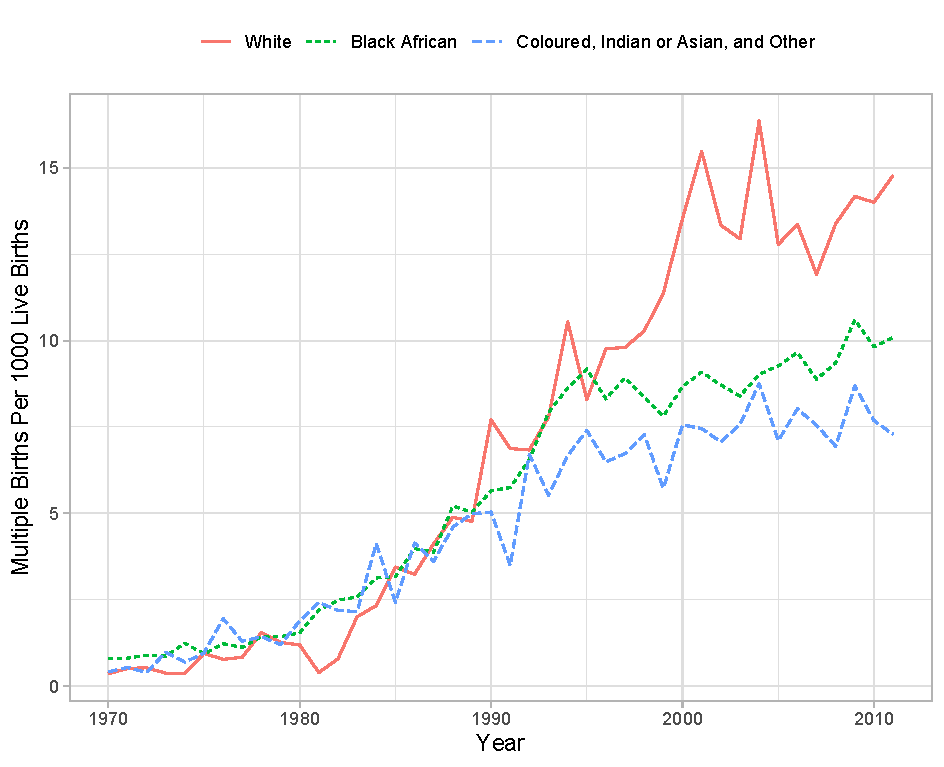
\includegraphics[width=\textwidth]{figures/line_pp.pdf}
%\end{figure}

%\begin{figure}[!th]
%\centering
%\caption{\label{fig:line-pp}Multiple Births Per 1000 Live Births by Mothers' Population Group}
%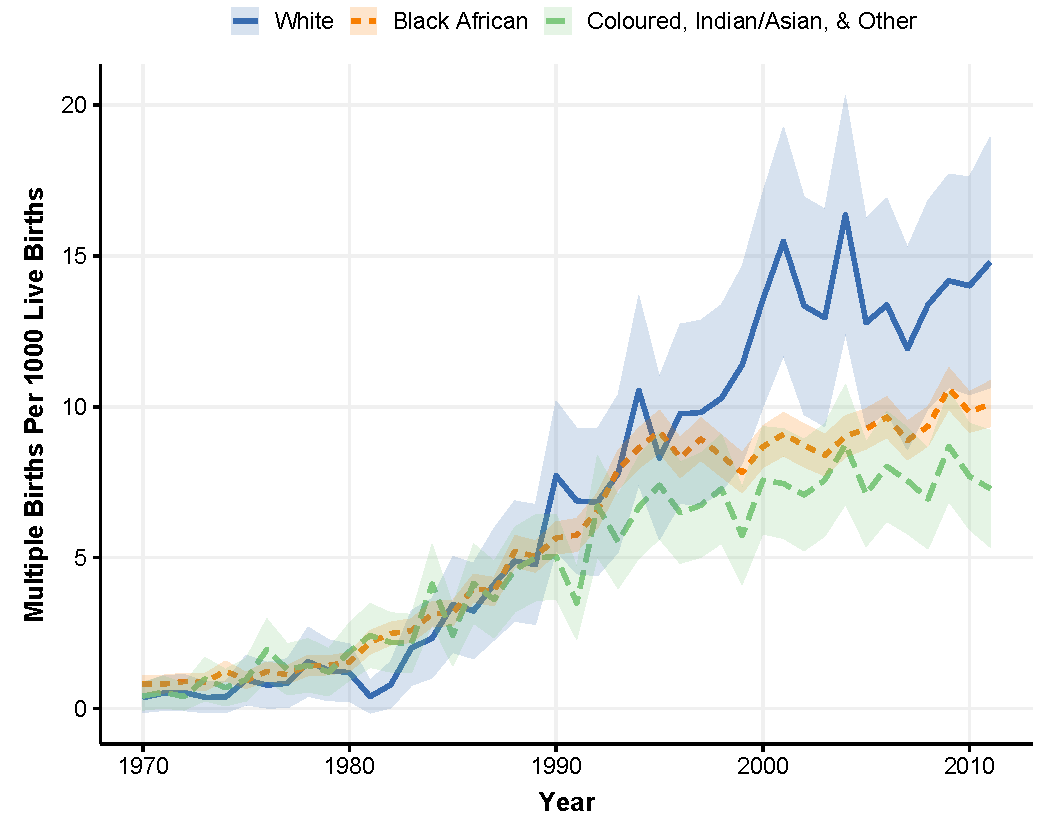
\includegraphics[width=\textwidth]{figures/line_rib.pdf}
%\fnote{\textit{Notes:} The solid lines represent the number of multiple births per 1000 live births for each population group, i.e., (number of multiple births/total birth)*1000. The ribbons are point-wise 95\% confidence intervals. The standard errors used to construct the confidence intervals were calculated using the following formula: se $ = 1000 \cdot \sqrt{p\cdot (1 - p)/n} $, where $ p $ is the proportion of multiple birth in a given year and $ n $ is the total number of live births. The formula assumes $ p $ follows the Bernoulli distribution.}
%\end{figure}
%\pagebreak

%
%Tex File: D:/R_projects/MScED_Dissertation/tex/tables/whites-nonwhites.tex

\begin{sidewaystable}[!htbp] \centering 
  \caption{Heterogeneity by Mother's Population Group (Whites vs. Non-Whites)} 
  \label{tab:whites-nonwhites} 
\begin{threeparttable}
\begin{tabular}{@{\extracolsep{8pt}}lcc@{\hskip 0.3in}cc@{\hskip 0.3in}cc@{\hskip 0.3in}cc} 
\\[-1.8ex]\hline 
\hline \\[-1.8ex] 
 & \multicolumn{4}{c}{2+ Sample} & \multicolumn{4}{c}{3+ Sample} \\
\cline{2-5}  \cline{6-9} \\
 & \multicolumn{2}{c}{Whites} & \multicolumn{2}{c}{Non-Whites} & 
    \multicolumn{2}{c}{Whites} & \multicolumn{2}{c}{Non-Whites} \\
\cline{2-3}  \cline{4-5} \cline{6-7} \cline{8-9} \\[-1.8ex]
\\[-1.8ex] & (1) & (2) & (3) & (4) & (5) & (6) & (7) & (8)\\ 
\hline \\[-1.8ex] 
\\[-2.0ex] \multicolumn{9}{@{} l}{\textbf{Panel A: First Stage$^{\dag}$}}
 \\
 \\[-1.5ex]
 Twins2/ & \multicolumn{2}{c}{ 0.942$^{***}$ }  & \multicolumn{2}{c}{ 0.809$^{***}$ } 
  &  \multicolumn{2}{c}{ 0.861$^{***}$ }  &  \multicolumn{2}{c}{ 0.756$^{***}$ }  \\ 
 Twins3 & \multicolumn{2}{c}{ (0.044) }  & \multicolumn{2}{c}{ (0.030) } 
  &  \multicolumn{2}{c}{ (0.068) }  &  \multicolumn{2}{c}{ (0.037) }  \\ 
 \multicolumn{1}{c}{$F$}  & \multicolumn{2}{c}{ [447.7] } & \multicolumn{2}{c}{ [732.5] } & \multicolumn{2}{c}{ [162.9] } & \multicolumn{2}{c}{ [422.2] } \\
\\[-1.83ex] 
 \hline \\[-1.83ex]
\\[-2.0ex] \multicolumn{9}{@{} l}{\textbf{Panel B: OLS \& 2SLS$^{\ddag}$}}
 \\
 \\[-1.5ex]
 & OLS & IV & OLS & IV & OLS & IV & OLS & IV \\
 \hline \\
 Educational Attainment & $-$0.001 & 0.019 & $-$0.005$^{***}$ & 0.003 & $-$0.009 & 0.026 & $-$0.007$^{***}$ & 0.011 \\ 
  & (0.002) & (0.012) & (0.001) & (0.007) & (0.005) & (0.018) & (0.001) & (0.010) \\ 
  & & & & & & & & \\ 
 Left Behind & 0.018$^{*}$ & $-$0.034 & 0.020$^{***}$ & $-$0.001 & 0.023 & $-$0.009 & 0.024$^{***}$ & $-$0.025 \\ 
  & (0.009) & (0.042) & (0.002) & (0.021) & (0.020) & (0.082) & (0.003) & (0.027) \\ 
  & & & & & & & & \\ 
 Private School & 0.021$^{**}$ & $-$0.010 & $-$0.004$^{***}$ & $-$0.017 & 0.047$^{*}$ & $-$0.094 & $-$0.004$^{***}$ & 0.015 \\ 
  & (0.007) & (0.035) & (0.001) & (0.011) & (0.019) & (0.081) & (0.001) & (0.015) \\ 
  & & & & & & & & \\ 
 Mothers LFP & $-$0.016$^{**}$ & 0.008 & $-$0.020$^{***}$ & $-$0.024 & $-$0.009 & 0.044 & $-$0.023$^{***}$ & 0.040 \\ 
  & (0.006) & (0.027) & (0.002) & (0.018) & (0.019) & (0.080) & (0.003) & (0.032) \\ 
  & & & & & & & & \\ 
\hline \\[-1.8ex] 
 $ N $  & \multicolumn{2}{c}{10,121} & \multicolumn{2}{c}{84,856} & \multicolumn{2}{c}{3,494} & \multicolumn{2}{c}{53,864} \\
\\[-2.0ex]
\hline 
\hline \\[-1.8ex] 
\end{tabular} 
\begin{tablenotes}
\footnotesize
\item \textit{Notes:} *** Significant at 1\%, ** Significant at 5\%, * Significant at 10\%. \\[-1.8ex] 

$ \dag $ Columns 1-4 have the coefficients for the Twins2
instrument (in the 2+ sample) and in columns 5-8 are the coefficients for the
Twins3 instrument (3+ sample). The regressions were run using the same set 
of controls as in \autoref{tab:main-res}. Robust standard errors are in parentheses and the numbers 
in square brackets below the s.e. are F stats for the exclusion of the Twins2 or
the Twins 3 variable from the model. \\[-1.8ex]
 
$ \ddag $ The regressions control for the same set of covariates as in \autoref{tab:main-res} (see notes there). 
The regressions for the 3+ sample are clustered by mother's ID. 

\end{tablenotes}
\end{threeparttable}
\end{sidewaystable} 



 
%\pagebreak

%\begin{figure}[!thbp]
%\centering
%\caption{\label{fig:hists}Histograms of Educational Attainment Index}
%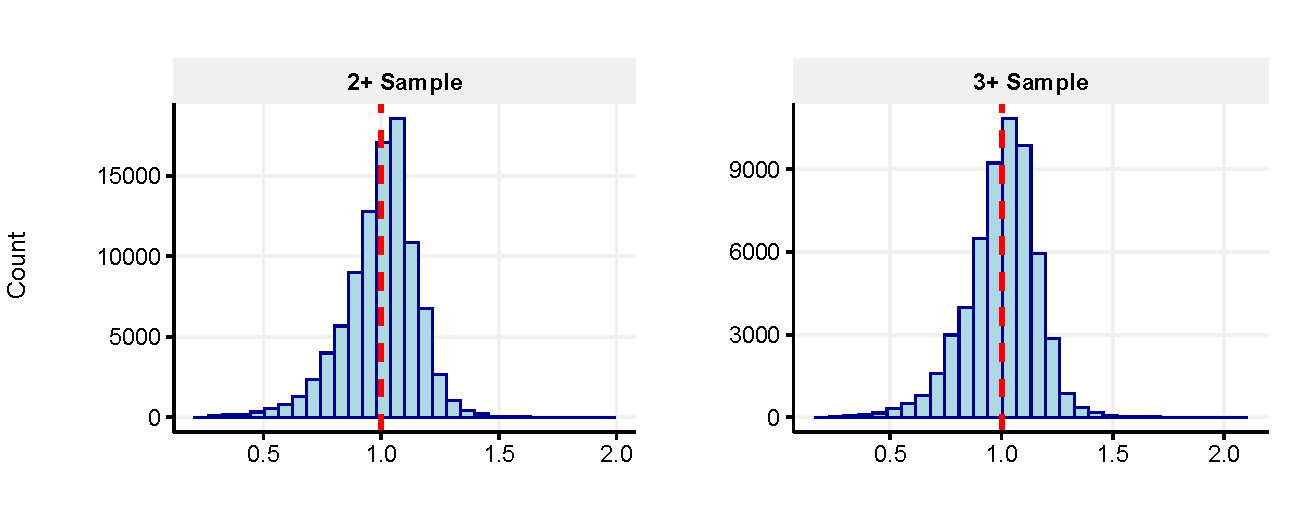
\includegraphics[width=0.93\textwidth]{figures/hists.pdf}
%\end{figure}


%Tex File: D:/R_projects/MScED_Dissertation/tex/tables/reduced.tex

\begin{table}[!htbp] \centering 
  \caption{Reduced Form Effects in No-First-Stage Samples} 
  \label{tab:reduced} 
\begin{threeparttable}
\begin{tabular}{@{\extracolsep{5pt}}lcccc} 
\\[-1.8ex]\hline 
\hline \\[-1.8ex] 
 & \multicolumn{2}{c}{Twins2$^{\dag}$} & \multicolumn{2}{c}{Boy12$^{\ddag}$} \\
 \cline{2-3} \cline{4-5} \\
 & Spacing $<$ 2 & No Schooling & Spacing $<$ 2 & No Schooling \\
\\[-1.8ex] & (1) & (2) & (3) & (4)\\ 
\hline \\[-1.8ex] 
\\[-2.0ex] \multicolumn{5}{@{} l}{\textbf{Panel A: First Stage}}
 \\
 \\[-1.5ex]
 No. of children & 0.266$^{*}$ & 0.101 & $-$0.0004 & 0.041 \\ 
  & (0.141) & (0.134) & (0.037) & (0.046) \\ 
  & & & & \\ 
\\[-1.83ex] 
 \hline \\[-1.83ex]
\\[-2.0ex] \multicolumn{5}{@{} l}{\textbf{Panel B: Reduced Form$^{\S}$}}
 \\
 \\[-1.5ex]
 Educational Attainment & 0.031 & 0.006 & 0.001 & 0.007 \\ 
  & (0.025) & (0.021) & (0.006) & (0.007) \\ 
  & & & & \\ 
 Left Behind & $-$0.131$^{*}$ & $-$0.067 & 0.013 & $-$0.026 \\ 
  & (0.070) & (0.067) & (0.018) & (0.020) \\ 
  & & & & \\ 
 Private School & 0.027 & $-$0.011$^{***}$ & 0.005 & 0.001 \\ 
  & (0.053) & (0.004) & (0.011) & (0.006) \\ 
  & & & & \\ 
 Mothers LFP & 0.033 & $-$0.052 & 0.034$^{**}$ & 0.005 \\ 
  & (0.065) & (0.067) & (0.015) & (0.020) \\ 
  & & & & \\ 
\hline \\[-1.8ex] 
 $ N $  & 3,489 & 3,022 & 2,869 & 2,381 \\
\hline 
\hline \\[-1.8ex] 
\end{tabular} 
\begin{tablenotes}
\footnotesize
\item \textit{Notes:} *** Significant at 1\%, ** Significant at 5\%, * Significant at 10\%. 
The same set of covariates as in \autoref{tab:main-res} were included in all regressions. Robust standard
errors in parentheses.
\\[-1.8ex]

$ \dag $ The subsamples are restricted to firstborns from families with at least three children.

$ \ddag $ Subsamples includes only firstborn boys.

$ \S $ In addition to the covariates used in \autoref{tab:main-res}, the reduced form regressions control for 
the number of children in the family.
\end{tablenotes}
\end{threeparttable}
\end{table} 




%\pagebreak


\newpage

% Reset the counter for figs. and tables in addendum
\setcounter{figure}{0} 
\renewcommand{\thefigure}{B.\arabic{figure}}
\setcounter{table}{0} 
\renewcommand{\thetable}{B.\arabic{table}}

\section{Addendum}

\subsection{The Average Causal Response (ACR) Framework}
\label{section:acr-detail}

Let $ Z_{i} $ be a binary instrument and let $ n_{i} $ be an endogenous variable that takes on the integer values $ \{0, 1, \dots, J\} $. Then there are $ J $ unit causal effects: the effect of going from 0 to 1, the effect of going from 1 to 2, \dots, and the effect of going from $ J-1 $ to $ J $. The average causal response (ACR) theorem says that the Wald estimator is a weighted average of the unit causal responses along the length of an appropriately defined response function (\parencite{Angrist2009,Angrist1995}). More formally, let $ N_{0i} $ and $ N_{1i} $ be the potential number of children in the family if the binary instrument $ Z_{i} $ were equal to 0 and 1, respectively. The observed number of children $ n_{i} $ is then, $ n_{i} = N_{0i} + (N_{1i} - N_{0i})\cdot Z_{i} $. Similarly let $ Y_{i}(j) $ be the potential outcome as a function of $ j $, where $ j $ takes possible values for $ n_{i} $ in the set $ \{0, 1, \dots, J\} $. Only one of these potential outcomes is realized and we denote the observed outcome by $ y_{i} $. In the simplest case with no covariates, the IV estimator using a binary instrument $ Z $ gives the Wald estimator.\footnote{The interpretation of the ACR is more elaborate when covariates are added, but the basic idea is preserved. See \textcite[p.~437]{Angrist1995}.} Then,

\begin{equation}\label{eq:02}
	\beta_{w} = \dfrac{\mathbb{E}(y_{i} | Z_{i} = 1) - \mathbb{E}(y_{i} | Z_{i} = 0)}{\mathbb{E}(n_{i} | Z_{i} = 1) - \mathbb{E}(n_{i} | Z_{i} = 0)} = \sum_{j = 1}^{J} \omega_{j}\cdot \mathbb{E}(Y_{i}(j) - Y_{i}(j-1) | N_{1i} \geq j > N_{0i}),
\end{equation}

where
\begin{equation}\label{eq:03}
\omega_{j} = \dfrac{\mathbb{P}(N_{1i} \geq j > N_{0i})}{\sum_{i = 1}^{J} \mathbb{P}(N_{1i} \geq i > N_{0i})}.
\end{equation}
\vskip10pt

The unit causal response in \eqref{eq:02}, $ \mathbb{E}(Y_{i}(j) - Y_{i}(j-1) | N_{1i} \geq j > N_{0i}) $, is the average difference in potential outcomes for \textit{compliers} at point $ j $; that is, individuals driven by the instrument from a treatment intensity less than $ j $ to at least $ j $. Thus, the Wald estimator, $ \beta_{w} $, is \enquote{a weighted ACR for people from families induced by an instrument to go from having fewer than $ j $ to at least $ j $ children, weighted over $ j $ by the probability of crossing this threshold} \parencite[p.~787]{angrist_multiple_2010}. The numerator in the expression for the weights $ \omega_{j} $ in \eqref{eq:03}, $ \mathbb{P}(N_{1i} \geq j > N_{0i}) $, represents the proportion of compliers at point $ j $.\footnote{Individuals with $ N_{1i} \geq j > N_{0i} $  for any $ j $ in the support of $ n_{i} $ are considered as compliers.} This is normalized by $ \sum_{i = 1}^{J} \mathbb{P}(N_{1i} \geq i > N_{0i}) $, which can be shown to be equal to the Wald first stage \parencite[see][p.~183]{Angrist2009}. That is,

\begin{equation}\label{eq:04}
\mathbb{E}(n_{i} | Z_{i} = 1) - \mathbb{E}(n_{i} | Z_{i} = 0) = \sum_{i = 1}^{J} \mathbb{P}(N_{1i} \geq i > N_{0i}).
\end{equation}

The size of the complier sub-population at each $ j $ can be estimated from the first stage regression. \autoref{fig:acrs} plots differences in the probability that the number of kids is at least as large as $ j $, as indicated in the x-axis labels. The coefficients and standard errors in the different panels are obtained by running a simple linear regression of a dummy for having at least $ j $ kids $ (j = 3, 4, \dots, 9) $ on the various instruments. The coefficients plotted provide an estimate of $ \mathbb{P}(N_{1i} \geq j > N_{0i}) $ for $ j = 3, 4, \dots, 9 $ and their sum is equal to the (unconditional) first stage coefficient (see \eqref{eq:04}), labeled as \enquote{overall}. For a given instrument, the size of the coefficient at a given parity, normalized by the overall first stage, is the weight attached to the unit causal effect at that parity. These weights reveal the extent to which an instrument causes a variation in family size at higher parities.  

There are three assumptions that lie behind the ACR theorem: (i) independence and exclusion; (ii) the existence of a valid first Stage; and (iii) monotonicity \parencite{Angrist2009}. The independence assumption requires that the instrument be independent of potential outcomes and potential treatment assignments. This is sometimes alternatively stated by saying that the instrument needs to be \enquote{as good as randomly assigned}. Both the twins and same sex instruments were originally proposed as natural experiments for fertility on the ground that both are virtually randomly assigned \parencite{rosenzweig_testing_1980,angrist_children_1998}. However, this is no longer obvious, because various threats to the randomness of both instruments have been pointed out in the literature (see Section~\ref{section:valid}). The exclusion assumption, on the other hand, says that the instrument used has no effect on the outcomes other than through its effect on family size.  Although this is closely related to the independence assumption, it is distinct from it. The exclusion restriction is a \enquote{a claim about a unique channel for causal effects of the instrument} \parencite[p.~153]{Angrist2009}. Again, various authors have pointed out ways in which exclusion restriction might fail to hold for both instruments. I have tried to address some of the important concerns in Section~\ref{section:valid}.

The other important assumption needed to estimate the ACR is monotonicity. In our case, monotonicity requires that the proposed instrument moves fertility in one direction only. In particular, we assume that the potential number of children when the instrument is switched on is at least as large as it would have been when it is switched off; i.e., $ N_{1i} \geq N_{0i} $. This is automatically satisfied by the twins instrument as fertility is always increased because of a twin birth for any mother. Although rare, it is possible that monotonocity might fail to hold for the same sex instrument. For example, there could be parents who prefer children of the same sex and therefore go on to have another child if the sexes of the first two or three children are different \parencite{Huber2015}. As a partial check on monotonicity, I estimated the same sex first stage in the 2+ sample for each combination of the mother's population group, intervals of the mother's age at first birth, and the level of education of the mother. Out of the 44 first stage regressions, corresponding to the 44 cells, only three generate negative estimates and all three were insignificant. The remaining significant estimates were all positive.

%The other important assumption needed to estimate the ACR is monotonicity. To understand the idea behind this assumption, we need to introduce the four mutually exclusive groups comprising of our quasi-experimental population: compliers, always takers, never takers, and defiers. These were first outlined in the treatment-effects framework of \textcite{angrist_identification_1996}.  Always takers always get treated regardless of their assignment, never takers never get treated regardless of their assignment, and compliers get treated when the instrument is switched on and don't get treated otherwise. The defiers, on the other hand, are a very strange group who get treated when the instrument is switched off and don't get treated when it is switched on. The assumption of monotonicity rules out the presence of defiers since they complicate the link between ACR and the reduced form \parencite{Angrist2009}.\footnote{\textcite{Angrist2009} discuss monotonicity in the context of the LATE framework of \textcite{imbens_identification_1994}. But this carries over directly to the ACR since the ACR is just an extension of the LATE \parencite[see][p.~181]{Angrist2009}.}  In other words, monotonicity rules out the case where the instrument pushes some people into treatment while pushing others out. In our case, monotonicity requires that the proposed instrument moves fertility in one direction only. In particular, we assume that the potential number of children when the instrument is switched on is at least as large as it would have been when it is switched off; i.e., $ N_{1i} \geq N_{0i} $. This is automatically satisfied by the twins instrument as fertility is always increased because of a twin birth for any mother. However, monotonicity need not hold for the same sex instrument as there could be parents who prefer children of the same sex and therefore go on to have another child if the sexes of the first two or three children are different \parencite{Huber2015}. In Section~\ref{section:samesx}, I discuss a partial check for monotonicity using first stage regressions. 

%\pagebreak

\begin{figure}[!ht]
\centering
\caption{\label{fig:acrs}Unconditional First-Stages and 95\% Confidence Intervals for Different Family Sizes}
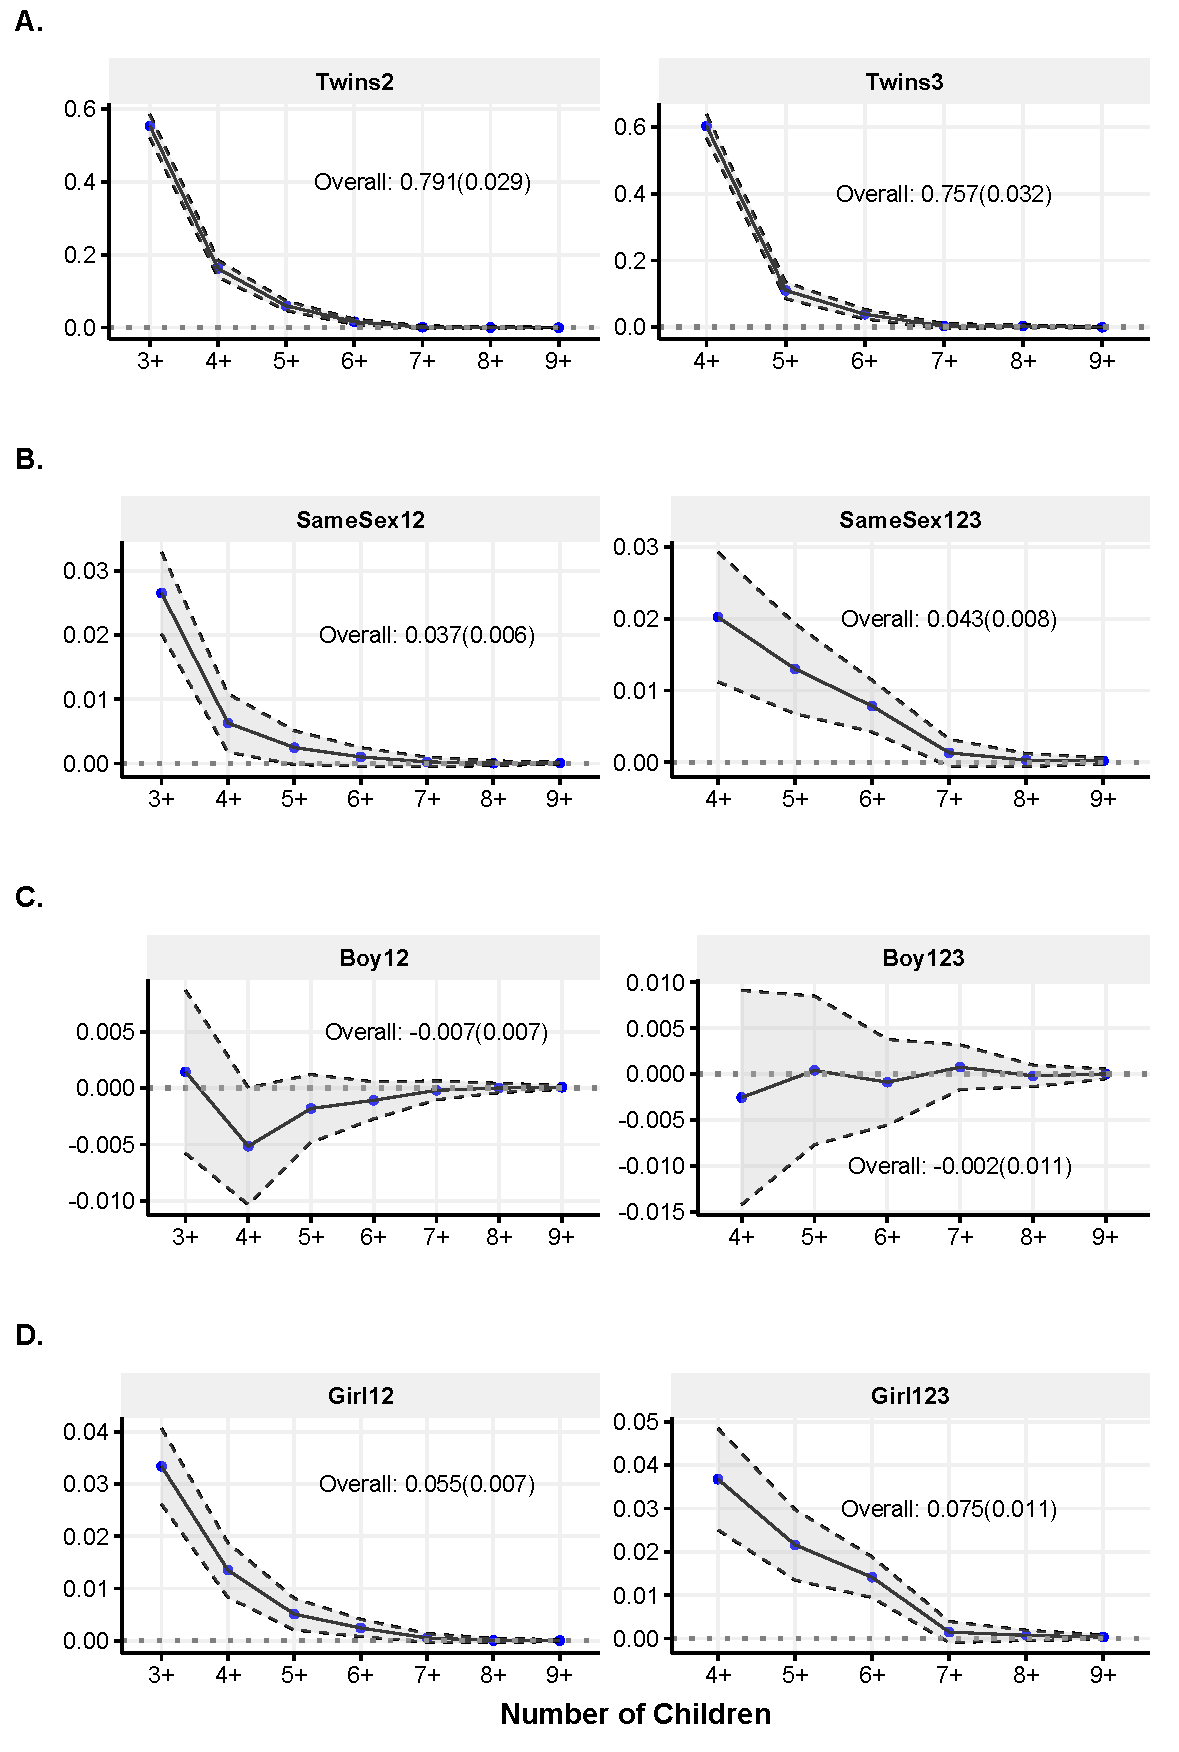
\includegraphics[width=\textwidth]{figures/acrs.pdf}
\fnote{\textit{Notes:} The coefficients and standard errors in the different panels are obtained by running a simple linear regression of a dummy for having at least $ j $ kids on the relevant instrument. Dashed lines are confidence bands. Overall first stages and standard errors are shown in the plot area.}
\end{figure}

%\pagebreak

\subsection{Generalized Random Forest Estimates}

\begin{figure}[p!]
\centering
\caption{\label{fig:heter1}Results of Generalized Random Forest Using Twins IV}
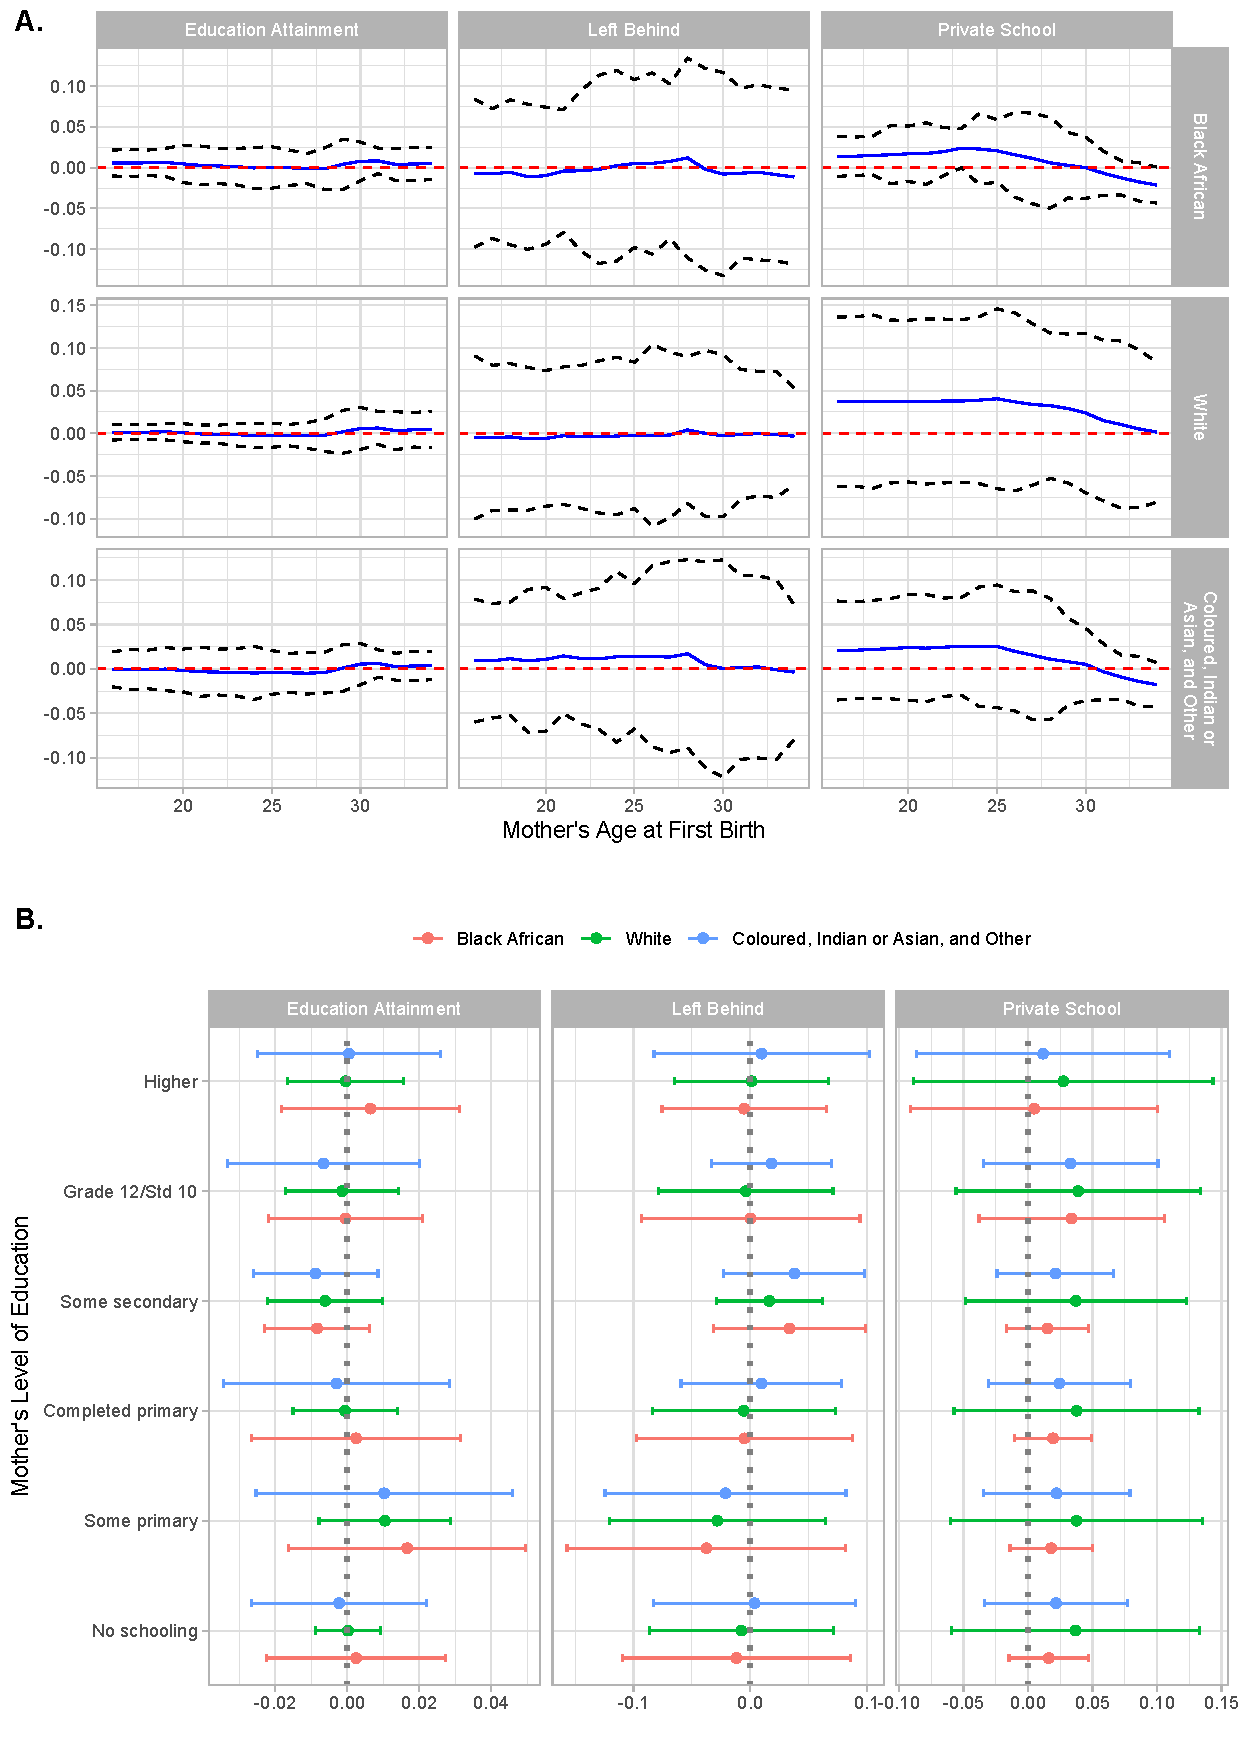
\includegraphics[width=\textwidth]{figures/heter1.pdf}
\fnote{\textit{Notes:} The above results are based on three forests, one forest for each outcome. Tuning results suggest the default values of the parameters as optimal for each forest: subsample fraction ($ s/n $) $ = 0.5 $, minimum leaf size ($ k $) $ = 5 $, number of splitting variables (\texttt{mtry}) $ = 26 $ (out of 33), balance parameter ($ \alpha $) $ = 0.05 $, and imbalance penalty $ = 0 $ (see the software implementation of \textcite{Athey2019} for the description of these parameters). Each forest is based on 5000 trees.}
\end{figure}
\pagebreak

\begin{figure}[p!]
\centering
\caption{\label{fig:heter2}Results of Generalized Random Forest Using Same-Sex IV}
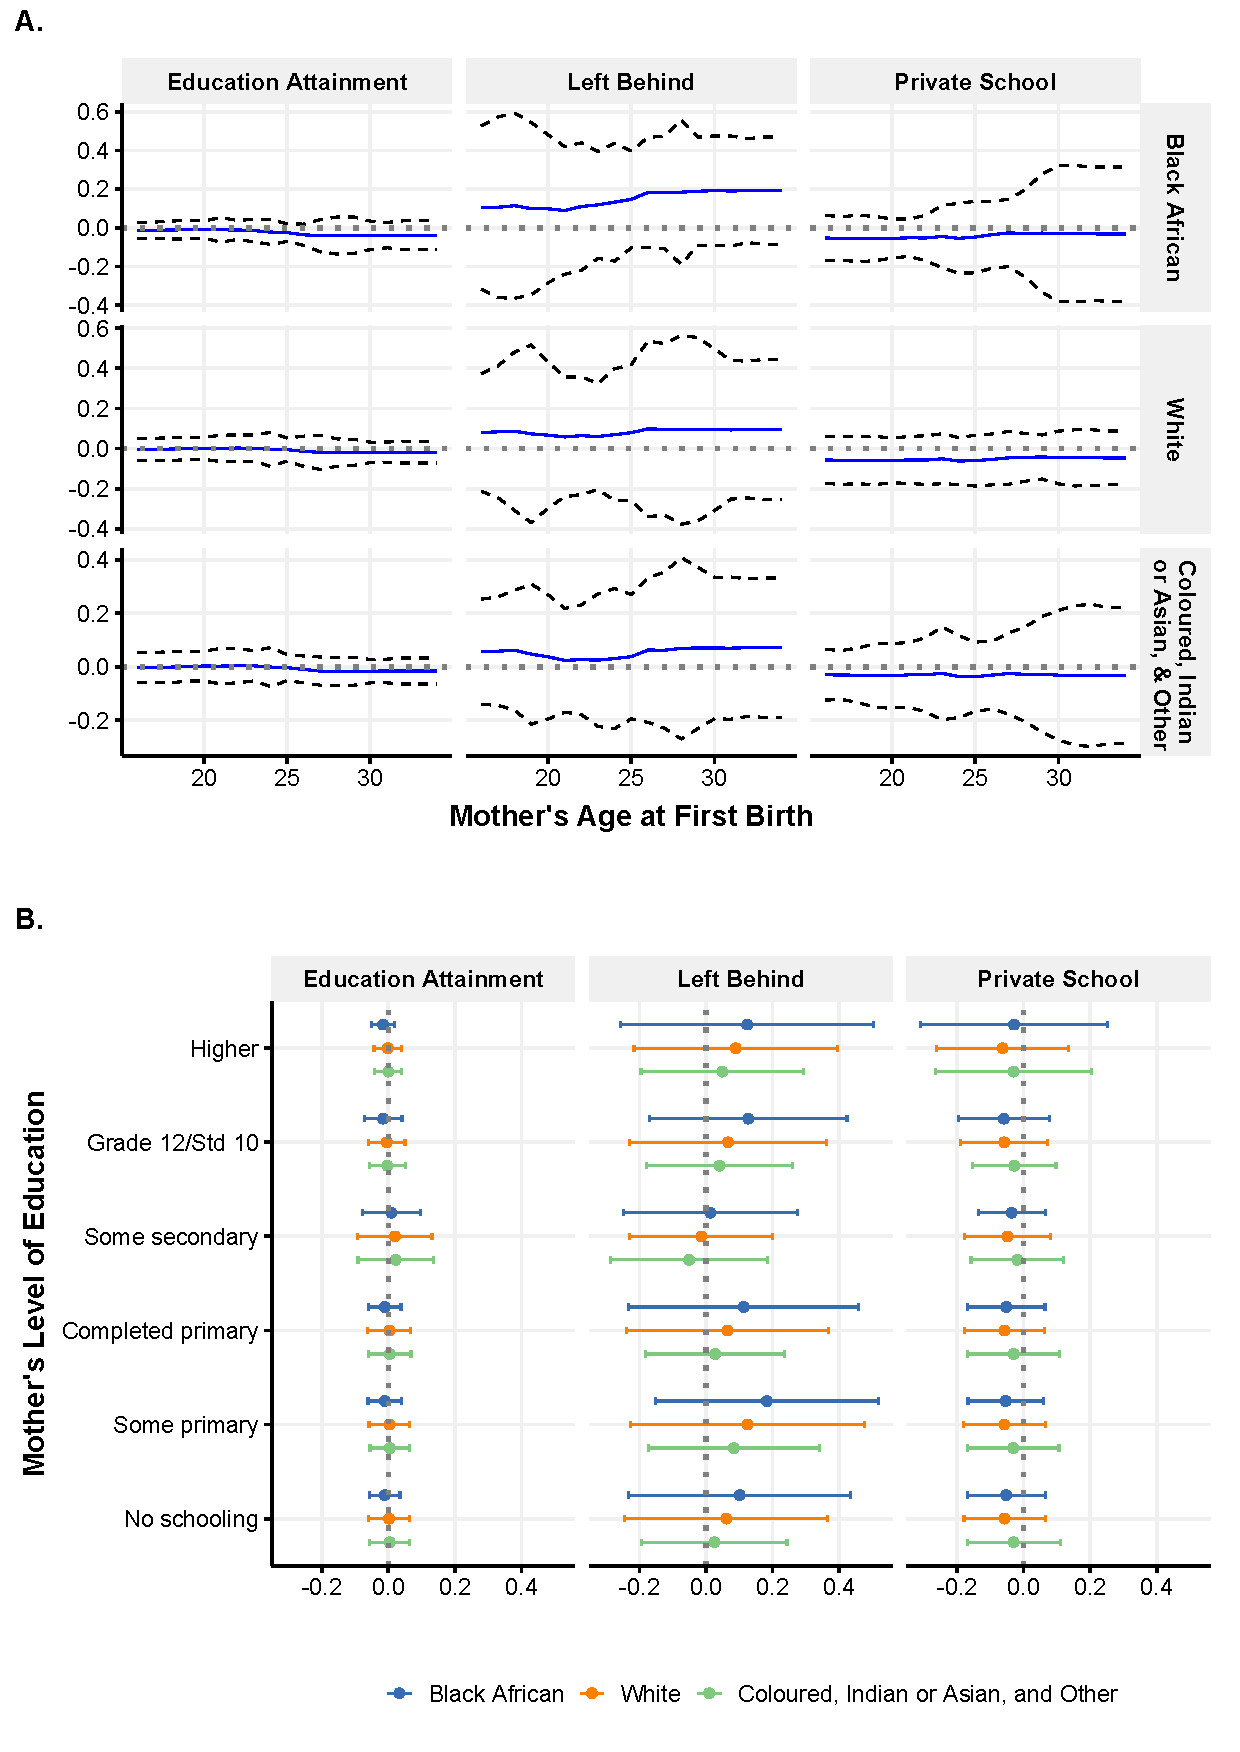
\includegraphics[width=\textwidth]{figures/heter2.pdf}
\fnote{\textit{Notes:} The above results are based on three forests, one forest for each outcome. The parameters supplied in training each forest were chosen by tuning based on cross-validation and are shown in the table below:
\centering
\begin{tabular}{rrrrrr}
  \hline
 & sample.fraction & mtry & min.node.size & alpha & imbalance.penalty \\ 
  \hline
educ & 0.25 & 7.00 & 53.00 & 0.21 & 0.55 \\ 
  behind & 0.08 & 8.00 & 71.00 & 0.07 & 1.26 \\ 
  private & 0.10 & 9.00 & 83.00 & 0.10 & 3.12 \\ 
   \hline
\end{tabular}
  Each forest is based on 5000 trees. }
\end{figure}
\pagebreak



% add se (CI) on the line graph
% Write/edit descriptions of figures and tables
% Build forest using 10000 trees (talk to Nati)
% Clean-up everything and archive.

\end{document}